\chapter{A Frequency Domain Investigation on the Morphology of the Solar Mean Magnetic Field}\label{chap:SMMF}

%%%%%%%%%%%%%%%%%%%%%%%%%%%%%%%%%%%%%%%%%%%%%%%%%%%%%%%%%%%%%%%%%%%%%
%%%%%%%%%%%%%%%%%%%%%%%%%%%%%%%%%%%%%%%%%%%%%%%%%%%%%%%%%%%%%%%%%%%%%

\textit{Most of the content in this chapter has been restructured for publication in the journal Monthly Notices of the Royal Astronomical Society \citep{ross_lifetimes_2021}. I was first author on this journal article and conducted the entirety of the work in the investigation.}

%%%%%%%%%%%%%%%%%%%%%%%%%%%%%%%%%%%%%%%%%%%%%%%%%%%%%%%%%%%%%%%%%%%%%
%%%%%%%%%%%%%%%%%%%%%%%%%%%%%%%%%%%%%%%%%%%%%%%%%%%%%%%%%%%%%%%%%%%%%
\section{Introduction}\label{sec:SMMF_intro}

The Sun has a complicated magnetic field structure; many features of the Sun and proxies for the solar activity are related to the evolution of the Sun's magnetic field \citep{wu_solar_2018}.

The \gls{smmf} is a surprising, non-zero measurement of the imbalance of opposite magnetic flux polarities observed on the full, visible disc of the Sun \citep{svalgaard_suns_1975}, and is defined as the mean \gls{los} magnetic field when observing the Sun-as-a-star \citep{scherrer_mean_1977, scherrer_mean_1977-1, garcia_integrated_1999}. In the literature the \gls{smmf} is also sometimes referred to as the \gls{gmf} \citep{severny_time_1971} or the \gls{mmf} \citep{kotov_mean_2008} of the Sun.

Observations of the \gls{smmf} have typically been made by measuring the Zeeman splitting of spectral lines using a ground-based Babcock-type magnetograph \citep{scherrer_mean_1977}, although more recently the \gls{smmf} has been calculated from full-disc \gls{los} magnetograms taken from space-borne telescopes such as the \gls{sdo/hmi}, in order to understand the morphology of the \gls{smmf} \citep{kutsenko_contribution_2017, bose_variability_2018}. It is understood that the strength of the \gls{smmf} may vary depending on the spectral line used to measure the \gls{smmf} \citep{kotov_mean_2008, kotov_enigmas_2012}; however, the SMMF varies slowly with the solar activity cycle, with an amplitude on the order of a Gauss during solar maximum and a tenth of a Gauss during solar minimum \citep{plachinda_general_2011}. In addition, the \gls{smmf} displays a strong, quasi-coherent rotational signal, which must arise from inhomogeneities on the solar disc with lifetimes of several rotations \citep{chaplin_studies_2003, xie_temporal_2017}.

Despite existing literature on \gls{smmf} observations spanning several decades, ultimately, the origin of the \gls{smmf} remains an open question in solar physics. The principle component of the \gls{smmf} is commonly assumed to be weak, large-scale magnetic flux, distributed over vast areas over the entire solar disc, rather than from more concentrated regions such as \glspl{ar} or sunspots \citep{severny_time_1971, scherrer_mean_1977, xiang_ensemble_2016}. However, conversely, \citet{scherrer_mean_1972} found that the \gls{smmf} was most highly correlated with flux from only the inner-most one quarter, by area, of the solar disc, which is more sensitive to active latitudes.

In recent literature, \citet{bose_variability_2018} provided a novel approach to understanding the \gls{smmf} whereby they decomposed the \gls{smmf} through feature identification and pixel-by-pixel analysis of full-disc magnetograms. \citet{bose_variability_2018} concluded that: (i) the observed variability in the \gls{smmf} lies in the polarity imbalance of large-scale magnetic field structures on the visible surface of the Sun, (ii) the correlation between the flux from sunspots and the \gls{smmf} is statistically insignificant, (iii) and more critically that the background flux dominates the \gls{smmf}, accounting for around $89 \%$ of the variation in the \gls{smmf}. However, there still remained a strong manifestation of the rotation in the background magnetic field presented by \citet{bose_variability_2018}. This is indicative of inhomogeneous magnetic features with lifetimes on the order of several solar rotations rather than the shorter-lived, weaker fields usually associated with the large-scale background. It therefore raises the question of whether their technique assigned flux from \glspl{mfc} or \glspl{ar} to the background.

In order to identify the contours of specific features \citet{bose_variability_2018} used an adaptive thresholding technique on various \gls{sdo/aia} images of the solar disc to create binary masks for different types of features. These masks were then applied to scaled \gls{sdo/hmi} magnetograms in order to separate the features on the disc and their contribution to the \gls{smmf}. Upon a closer inspection of the example magnetogram in Figure 2 of the paper (shown in Figure~\ref{fig:bose_fig2}), with over-plotted contours of identified features from \gls{sdo/aia} images, there are clearly regions of strong \glspl{mfc} in the local vicinity of, and connected to, the identified features that lie outside their contour lines. Therefore these were allocated to the background magnetic field, rather than attributed to the specific features. It seems an obvious statement to suggest that \gls{sdo/aia} optical counterparts of the magnetograms will not exactly align with the observed magnetic flux in the magnetograms. We expect that the magnetic field will manifest itself differently in the optical observations and the magnetograms, which leads one to believe that the background component in this study could mistakenly contain flux from some of the identified features.


\begin{figure}[ht!]
	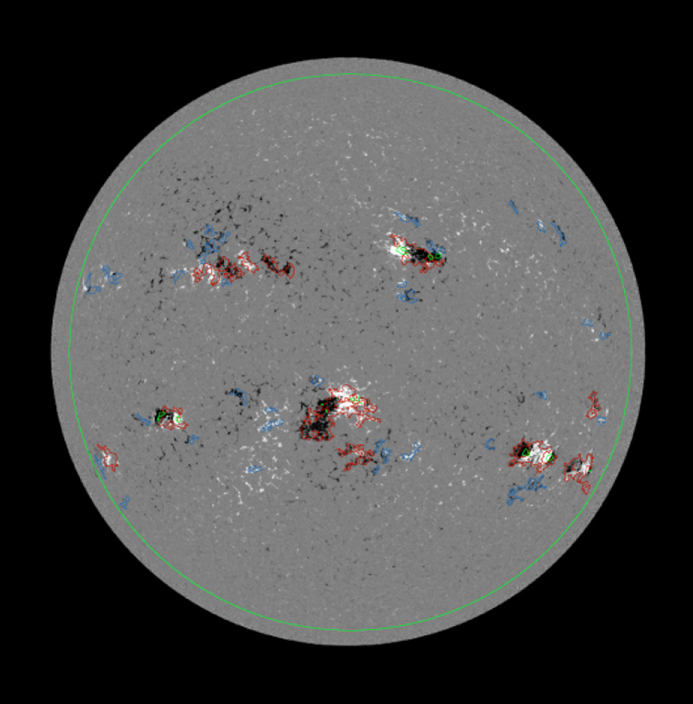
\includegraphics[width=\columnwidth]{bose_nag_plot.jpg}
	\caption{Figure 2 from \citet{bose_variability_2018}. The image shows a full-disc magnetogram of the Sun observed on 21-Apr-2012 00:00:00 UTC by SDO/HMI with the contours of the identified features over-plotted. The contours denote plages (red), enhanced networks (blue), sunspots (green). The circular fluorescent green contour depicts the solar disc within 0.97 $R_\odot$.}
	\label{fig:bose_fig2}
\end{figure}



In particular, in their example plot, the contours for sunspots typically only cover the umbra, not accounting for the surrounding penumbra. It is not clear whether this will have a large effect, but certainly we expect that some strong magnetic flux associated with sunspots has been attributed to the background, or other nearby features. One other note; there was a treatment of plages in this work, from additional chromospheric observations, but a separate, specific handling of faculae in the photosphere was absent. Incorporating this could have contributed to the completeness of the study. Furthermore, a decomposition of the identified background component into regimes of strong and weak field would have provided more clarity on the exact morphology of the \gls{smmf}, and would have likely provided evidence to conclude whether flux from \gls{ar} features were, in fact, incorporated into the background.

Despite these findings, it is known that the strength of the \gls{smmf} is weaker during solar minimum, when there are fewer \glspl{ar}, and stronger during solar maximum, when there are more \glspl{ar}. This is suggestive that the evolution of \glspl{ar} has relevance for the evolution of the \gls{smmf}.

There is a contrasting view in the literature which suggests \gls{ar} flux dominates the \gls{smmf}. \citet{kutsenko_contribution_2017} claim that a large component of the \gls{smmf} may be explained by strong and intermediate flux regions. These regions are associated with \glspl{ar}; using a thresholding technique they showed between $65 \%$ to $95 \%$ of the \gls{smmf} could be attributed to strong and intermediate flux, while the fraction of the occupied area varied between $2 \%$ to $6 \%$ of the disc area, depending on the chosen threshold for separating weak and strong flux. This finding suggests that strong, long-lived, inhomogeneous \gls{mfc}s produce the strong rotation signal in the \gls{smmf}. Potential sources could be sunspots, plages, faculae, etc. and \citet{kutsenko_contribution_2017} stated that there is an entanglement of strong flux (typically associated with \glspl{ar}) and intermediate flux (typically associated with network fields and remains of decayed \glspl{ar}). Disentangling the flux would have provided a more accurate analysis of the \gls{smmf}, owing to a clearer picture of the main contributor to the \gls{smmf}.

The Sun's dynamo and hence magnetic field is directly coupled to the solar rotation. The Sun exhibits latitude-dependent and depth-dependent differential rotation with a sidereal, equatorial period of around 25~days \citep{howe_solar_2009}. To Earth-based observers, the synodic rotation of the Sun is observed at around 27~days, and the \gls{smmf} displays a dominant periodicity of around 27~days due to the solar rotation \citep{chaplin_studies_2003, xie_temporal_2017, bose_variability_2018}. It was also reported by \citet{xie_temporal_2017} that the surface differential rotation was observed in the \gls{smmf} with measured rotational periods of $28.28 \, \pm \, 0.67$~days and $27.32 \, \pm \, 0.64$~days for the rising and declining phases, respectively, of all of the solar cycles in their considered time-frame.

On the other hand, \citet{xiang_ensemble_2016} utilised ensemble \gls{eemd} analysis to extract rotational modes in the \gls{smmf} and found two rotation periods which are derived from different strengths of magnetic flux elements. They found that a rotation period of 26.6~days was related to a weaker magnetic flux element within the \gls{smmf}, while for stronger magnetic flux elements in the \gls{smmf}, the measured rotation period was 28.5~days.

Ultimately, to date, our understanding of the \gls{smmf} and its origin remains open to question.


%%%%%%%%%%%%%%%%%%%%%%%%%%%%%%%%%%%%%%%%%%%%%%%%%%%%%%%%%%%%%%%%%%%%%
%%%%%%%%%%%%%%%%%%%%%%%%%%%%%%%%%%%%%%%%%%%%%%%%%%%%%%%%%%%%%%%%%%%%%
\section{Aims}\label{sec:SMMF_aims}

In this work an investigation of high-cadence (sub-minute) observations of the \gls{smmf}, made by \gls{bison} \citep{chaplin_bison_1996, chaplin_noise_2005, hale_performance_2016}, was performed. The aim of the investigation was to understand the morphology of the \gls{smmf}. 

This work provides a frequency domain analysis of the \gls{smmf} data, where a model was built and fit to the power spectrum of the \gls{smmf} which allowed us to understand the characteristics of its source(s). 

The \gls{rm} signal in the \gls{smmf} was clearly observed as several low-frequency peaks in the power spectrum. In addition, the use of the high-cadence data was especially crucial for inferences on components of the \gls{smmf} with periods of less than a day at higher frequencies in the power spectrum, with the intention to determine whether the background magnetic field exhibited a stochastically excited component, which evolved on short timescales.

%After fitting a model of the power spectrum, we aimed to use simulated data and other sources of \gls{smmf} data to aid the clarification of our inferences from \gls{bison} against other observations.



%%%%%%%%%%%%%%%%%%%%%%%%%%%%%%%%%%%%%%%%%%%%%%%%%%%%%%%%%%%%%%%%%%%%%
%%%%%%%%%%%%%%%%%%%%%%%%%%%%%%%%%%%%%%%%%%%%%%%%%%%%%%%%%%%%%%%%%%%%%
\section{Data}\label{sec:SMMF_data}


%%%%%%%%%%%%%%%%%%%%%%%%%%%%%%%%%%%%%%%%%%%%%%%%%%%%%%%%%%%%%%%%%%%%%
\subsection{Summary of the Data Set}

\citet{chaplin_studies_2003} provided the first examination of the \gls{smmf} using data from \gls{bison}, and the work presented in this paper is a continuation of that study.

\gls{bison} is a six-station, ground-based, global network of telescopes continuously monitoring the Sun, which principally makes precise measurements of the \gls{los} velocity of the photosphere due to solar $p$ mode oscillations \citep{hale_performance_2016}. Through the use of polarising optics and additional electronics, the \gls{bison} spectrometers can measure both the disc-averaged \gls{los} velocity and magnetic field in the photosphere \citep{chaplin_studies_2003}, however, not all \gls{bison} sites measure the \gls{smmf}. %The observing regime for \gls{bison} is described below.

In this study we focus on the data collected by the Sutherland node, in South Africa, which was also used by \cite{chaplin_studies_2003}. Data are sampled on a 40-second cadence, and the \gls{smmf} data collected by the Sutherland station pertains to the epochs from 01/1992 -- 12/2012 (i.e. covering 7643~days). Over this period, the fill (i.e. duty cycle) of solar observations is low because of the combination of: (a) the fill due to using only a single site with a 40-second cadence, (b) the duty cycle needed in a given day for a `good measure' of the Sun. Over this period, the average duty cycle of the 40-second data is $\sim$15.6\%. If instead we take a daily average of the \gls{bison} \gls{smmf}, the average duty cycle is $\sim$55.2\%. This gives a higher duty cycle but a lower Nyquist frequency. Because of the much lower Nyquist frequency, modelling the background power spectral density is more challenging; therefore we use the 40-second cadence data in this work.

As a comparison to the \gls{bison} data, \gls{smmf} observations were also acquired by the \gls{wso} (\url{http://wso.stanford.edu/}) \citep{scherrer_mean_1977-1}. The \gls{wso} \gls{smmf} data are sampled daily from 16/05/1975 -- present day, but for comparison with the \gls{bison} \gls{smmf}, we only used data over the same temporal range.

The \gls{wso} also measures the \gls{los} \gls{smmf} using a Babcock-type magnetograph, which allows the measurement of the amount and sense of circular polarisation in the wings in an absorption line \citep{scherrer_mean_1977}. \gls{wso} uses two absorption lines for the measurement of the magnetic field: the Fe I at 5250~\AA ($\lambda 5250$) is used for measurement of the field, and Fe I at 5124~\AA ($\lambda 5124$) is used to determine the instrument's zero offset, as this line is magnetically insensitive. \cite{scherrer_mean_1977} describes that a single, complete observation takes $\sim$20 minutes, consisting of four 3-minute integrations. The data provided by \gls{wso} are a daily weighted mean of the observations, where the weighting used is the statistical uncertainty and the magnitude of the zero offset measured with the $\lambda 5124$ line.


%%%%%%%%%%%%%%%%%%%%%%%%%%%%%%%%%%%%%%%%%%%%%%%%%%%%%%%%%%%%%%%%%%%%%
\subsection{Obtaining the SMMF from BiSON}

There is no catalogued \gls{bison} \gls{smmf} data-set, so it was necessary to compute the \gls{smmf} from the available \gls{bison} data. To acquire the \gls{smmf} from \gls{bison} data, the method as described by \citet{chaplin_studies_2003} was adopted; here we discuss the key aspects.

Each \gls{bison} site employs a \gls{rss} to measure the Doppler shift of the $^{2}\mathrm{S}_{1/2} \, \rightarrow \, ^{2}\mathrm{P}_{1/2}$ line (D1 line) of potassium, at $\sim$770~nm \citep{brookes_resonant-scattering_1978}. A potassium vapour cell placed within a longitudinal magnetic field Zeeman splits the laboratory line into the two allowed D1 transitions \citep{lund_spatial_2017}. The intensity of the longer wavelength (red; $I_R$) and shorter wavelength (blue; $I_B$) components of the line may be measured by the \gls{rss} almost simultaneously, by using polarising optics to switch between the red and blue wings of the line, to form the ratio given by equation~(\ref{eq:ratio}), which is used as a proxy for the Doppler shift from the \gls{los} velocity of the photosphere \citep[see:][]{brookes_observation_1976, brookes_resonant-scattering_1978, elsworth_performance_1995, chaplin_studies_2003, lund_spatial_2017}: 
%
\begin{equation}
\mathcal{R} = \frac{I_B - I_R}{I_B + I_R} \, .
\label{eq:ratio}
\end{equation}

%There are known effects which occur when making observations of the entire solar disc at one time, such as \gls{los} Doppler-imaging and limb-darkening \citep{davies_bison_2014}. Some \gls{bison} stations, that do not measure the \gls{smmf}, use optics to spatially scramble incoming sunlight to remove Doppler-imaging effects, to ensure a more accurate measure of the disc-averaged Sun-as-a-star. Sutherland, however, is not free from these effects, but they are assumed to be small in the analysis.

Photospheric magnetic fields Zeeman split the Fraunhofer line and the Zeeman-split components have opposite senses of circular polarisation \citep{chaplin_studies_2003}. Additional polarising optics are used in the \gls{rss} to manipulate the sense of circular polarisation (either + or -) that is passed through the instrument. The ratio $\mathcal{R}_{+}$ or $\mathcal{R}_{-}$ is formed, and the ratios $\mathcal{R}_{\pm}$ would be equal if there was no magnetic field present.

The observed ratio ($\mathcal{R}_{\pm}$) may be decomposed as:
%
\begin{equation}
\mathcal{R}_{\pm} = \mathcal{R}_{\mathrm{orb}} + \mathcal{R}_{\mathrm{spin}} + \mathcal{R}_{\mathrm{grs}} + \delta {r}_{\mathrm{osc}}(t) \pm \delta {r}_{\mathrm{B}}(t) \, ,
\label{eq:vel_comp}
\end{equation}
%
where $\mathcal{R}_{\mathrm{orb}}$ is due to the radial component of the Earth's orbital velocity around the Sun, $\mathcal{R}_{\mathrm{spin}}$ is due to the component towards the Sun of the Earth's diurnal rotation about its spin axis as a function of latitude and time, $\mathcal{R}_{\mathrm{grs}}$ is from the gravitational red-shift of the solar line due to the Sun's mass \citep{elsworth_techniques_1995, dumbill_observation_1999}, $\delta {r}_{\mathrm{osc}}(t)$ is due to the \gls{los} velocity of $p$ mode oscillations, and $\delta {r}_B(t)$ is due to the magnetic field ($\pm$ denotes the polarity of the Zeeman-split line that is being observed) \citep{dumbill_observation_1999}. 

%It is worth noting here that because of the inclusion of the $\pm$, it may appear that we're not sensitive to the sign of the magnetic field ($\delta {r}_{\mathrm{B}}(t)$); however, this is not the case. The magnetic field sign is measured, and the $\pm$ simply denotes the polarity of the Zeeman split line that is being observed.

%The \gls{los} velocity due to $p$ mode oscillations are given by , and . 

The effect of the magnetic field on the ratio is shown in Figure~\ref{fig:ratio_split}, and it is clear to see from equation~(\ref{eq:R_diff}) that the difference between the opposite magnetic field ratios is twice the magnetic ratio residual, i.e.:
%
\begin{equation}
\mathcal{R}_{+} - \mathcal{R}_{-} = 2 \, \delta {r}_{\mathrm{B}}(t) \, .
\label{eq:R_diff}
\end{equation}

\begin{figure}[ht!]
	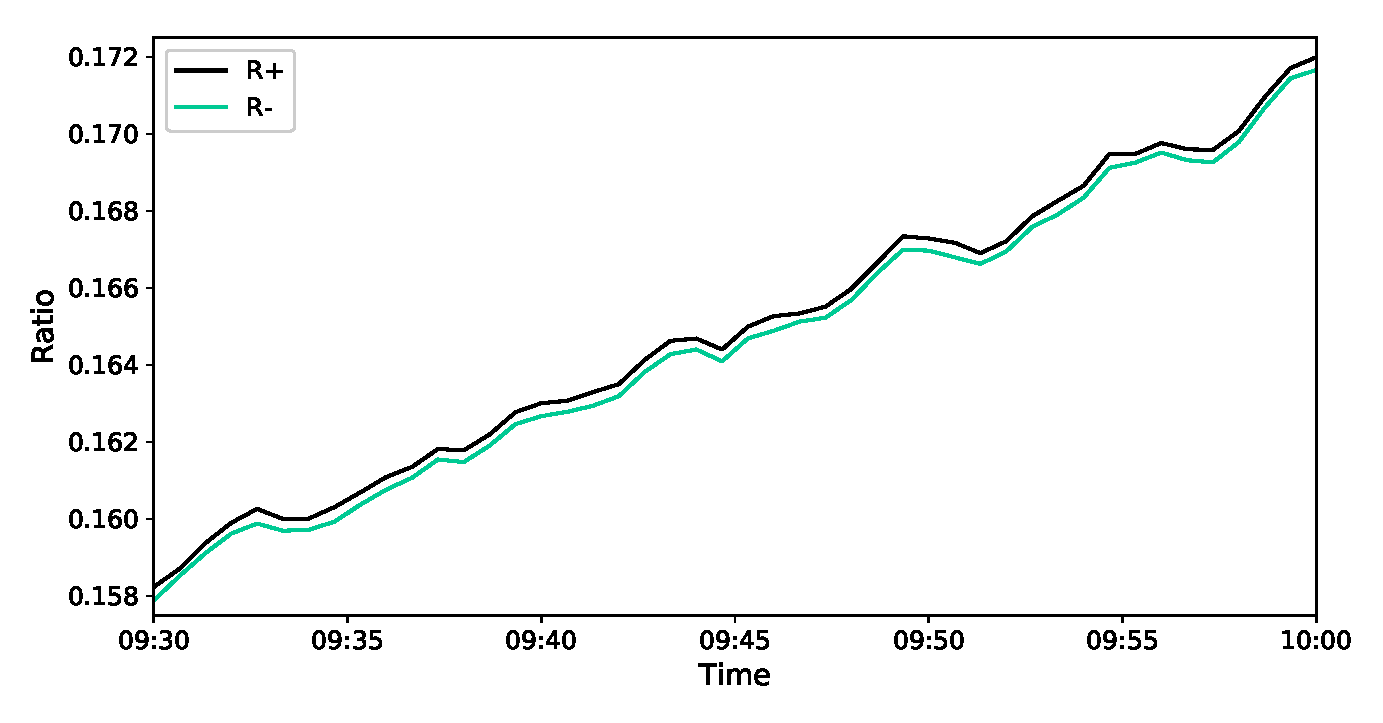
\includegraphics[width=\columnwidth]{Fred_ratio_zoom.eps}
	\caption{An example of the BiSON ratios data over a 30-minute period. The separation between the two ratios is due to the solar mean magnetic field. Other excursions in the individual ratios are due to the other effects measured by the RSS.}
	\label{fig:ratio_split}
\end{figure}

The \gls{bison} \gls{rss} is measuring the velocity variation on the solar disc, and therefore a calibration from the ratio to a velocity is necessary. One method of velocity calibration is achieved by first fitting the daily observed ratio, averaged over both magnetic polarities, to a 2nd- or 3rd-order polynomial as a function of velocity, as discussed by \citet{elsworth_techniques_1995}. Here we chose to fit the ratio in terms of velocity, $\mathcal{R}_{\mathrm{calc}}(u)$, i.e.:
%
\begin{equation}
\mathcal{R}_{\mathrm{calc}}(u) = \sum_{n} \mathcal{R}_{n} u^n \, ,
\label{eq:calc_ratio}
\end{equation}
%
where:
%
\begin{equation}
u = v_{\mathrm{orb}} + v_{\mathrm{spin}} \, ,
\label{eq:stn_vel}
\end{equation}
%
and $v_{\mathrm{orb}}$ is the velocity component related to the ratio,  $\mathcal{R}_{\mathrm{orb}}$; $v_{\mathrm{spin}}$ is related to the ratio, $\mathcal{R}_{\mathrm{spin}}$; and $n$ is the polynomial order.

It is possible to see that through the removal of $\mathcal{R}_{\mathrm{calc}}(u)$ from the observed ratios, one is left with the ratio residuals of the $p$ mode oscillations and the magnetic field, i.e.:
%
\begin{equation}
\mathcal{R}_{\pm} - \mathcal{R}_{\mathrm{calc}}(u) = \delta {r}_{\mathrm{osc}}(t) \pm \delta {r}_{\mathrm{B}}(t)
\label{eq:ratio_resid} \, .
\end{equation}

Furthermore, conversion from ratio residuals into velocity residuals uses the calibration given by:

\begin{equation}
\delta v(t) = \left( \frac{d\mathcal{R}_{calc}}{dV} \right)^{-1} \, \delta {r}(t) \, .
\label{eq:vel_resid}
\end{equation}

In order to finally obtain the \gls{smmf} in magnetic field units, one must combine equation~(\ref{eq:R_diff}) and  equation~(\ref{eq:vel_resid}) with the conversion factor in equation~(\ref{eq:K_B}) \citep{dumbill_observation_1999}, and the entire procedure can be simplified into:
%
\begin{equation}
B(t) = \frac{1}{2} \left( \frac{d\mathcal{R}_{calc}}{dV} \right)^{-1} \frac{(\mathcal{R}_{+} - \mathcal{R}_{-})}{K_B} \, ,
\label{eq:simplified_SMMF_cal}
\end{equation}
%
where:
%
\begin{equation}
K_B = \frac{8}{3} \, \frac{\mu_B}{h} \, \frac{c}{\nu} \approx 2.89 \, \mathrm{ms}^{-1} \, \mathrm{G}^{-1} \, ,
\label{eq:K_B}
\end{equation}
%
and $\mu_B$ is the Bohr magneton, $h$ is Planck's constant, $c$ is the speed of light, and $\nu$ is the frequency of the photons.

\begin{figure}[ht!]
	\centering
	\subfloat[BiSON SMMF 40-second cadence time series \label{fig:SMMF_TS}]{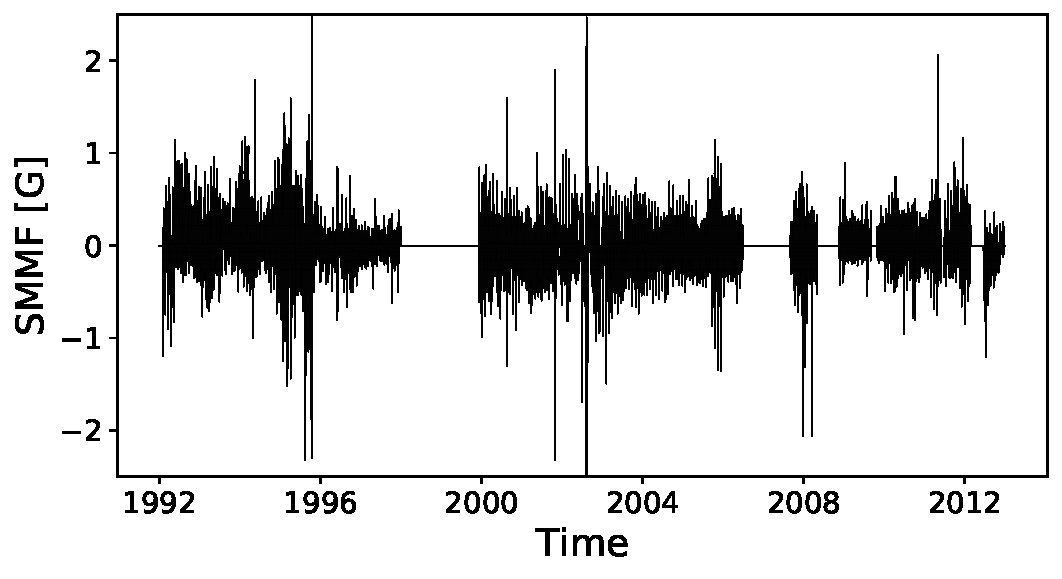
\includegraphics[width=0.99\columnwidth]{BiSON_full_TS.pdf}} \\ 
	\centering
	\subfloat[Power spectral density of the BiSON SMMF \label{fig:SMMF_FT}]{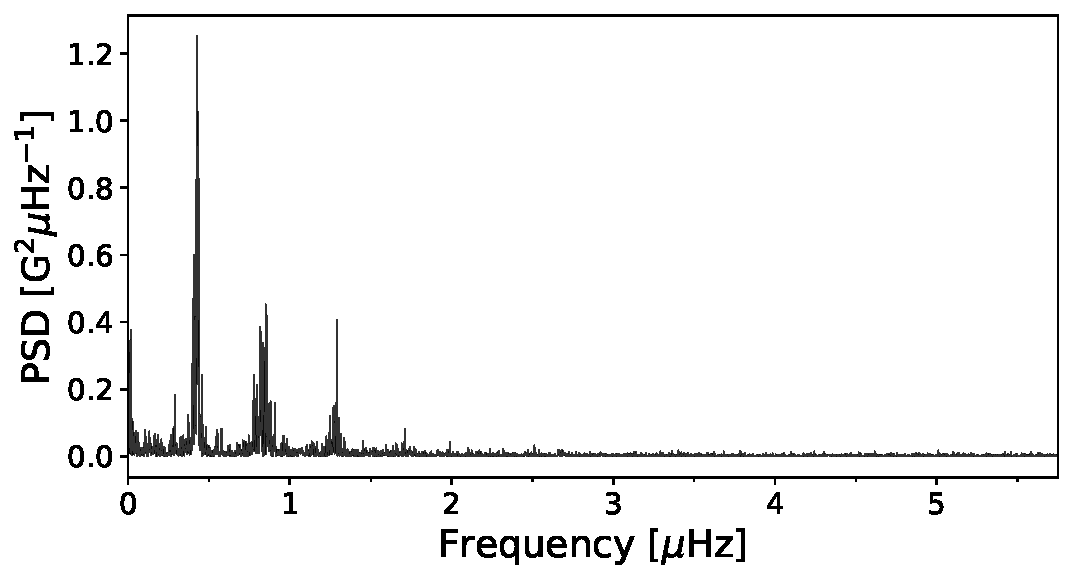
\includegraphics[width=\columnwidth]{BiSON_lin_mu_PSD.pdf}}
	\caption{(a) 40-second cadence observations of the SMMF from the Sutherland BiSON station between 1992 and 2012. The sense of the field was chosen to match the \citet{chaplin_studies_2003} and the WSO observations, where positive is for a field pointing outwards from the Sun. (b) Power spectrum of the SMMF on a 40-second cadence truncated to $10 \upmu\mathrm{Hz}$, however, the Nyquist frequency is $12500 \upmu\mathrm{Hz}$.}  
	\label{fig:BiSON_SMMF}
\end{figure}

Through the application of this methodology, one acquires the \gls{smmf} as shown in Figure~(\ref{fig:SMMF_TS}). The power spectrum of the full, 7643-day Sutherland data set is shown in Figure~(\ref{fig:SMMF_FT}). The power spectrum shows a clear set of strong peaks at low frequency, which are due to the persistent rotation signal in the \gls{smmf}. The largest peak is the fundamental rotation frequency, and the following peaks are its harmonics.


%%%%%%%%%%%%%%%%%%%%%%%%%%%%%%%%%%%%%%%%%%%%%%%%%%%%%%%%%%%%%%%%%%%%%%
%\subsection{Comparison between WSO and BiSON}
%
%The relationship between the \gls{smmf} measured by the Sutherland \gls{bison} node and the \gls{smmf} measured by Stanford \gls{wso} was examined. The daily \gls{smmf} measured by the Stanford \gls{wso} and Sutherland \gls{bison} station are plotted in Fig~\ref{fig:BiSON_and_WSO}.
%
%\begin{figure}[ht!]
%    \centering
%	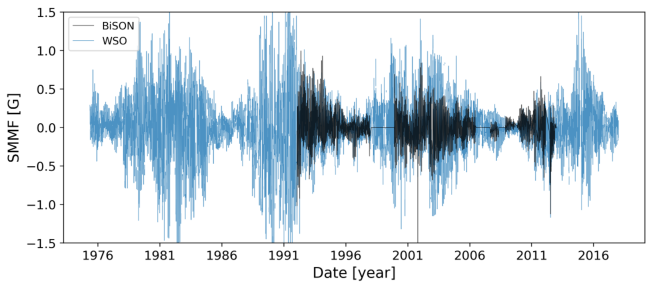
\includegraphics[width=\columnwidth]{BiSON_and_WSO.pdf}
%    \caption{Daily averaged SMMF measured by WSO (blue) and by the Sutherland BiSON station (black).}
%    \label{fig:BiSON_and_WSO}
%\end{figure}
%
%Figure~\ref{fig:BiSON_vs_WSO} shows the correlation between the two data sets, and also a comparison of their power spectra at low frequencies. The gradient of the line in Figure~\ref{fig:BiSON_vs_WSO_TS} is $0.4999\pm0.0001$ and informs us that the \gls{bison} \gls{smmf} is half of the magnitude of that observed by \gls{wso}. Interestingly \citet{chaplin_studies_2003} stated that the \gls{smmf} observed by the Sutherland \gls{bison} station was roughly twice that of \gls{wso}, which means there is a self-consistency problem with the calibration of the \gls{bison} \gls{smmf} and suggests that there is a factor of 4 difference between the measurements of the \gls{smmf} by \citet{chaplin_studies_2003} and in this work.
%
%\begin{figure}[ht!]
%	\centering
%	\subfloat[BiSON vs WSO correlation \label{fig:BiSON_vs_WSO_TS}]
%	{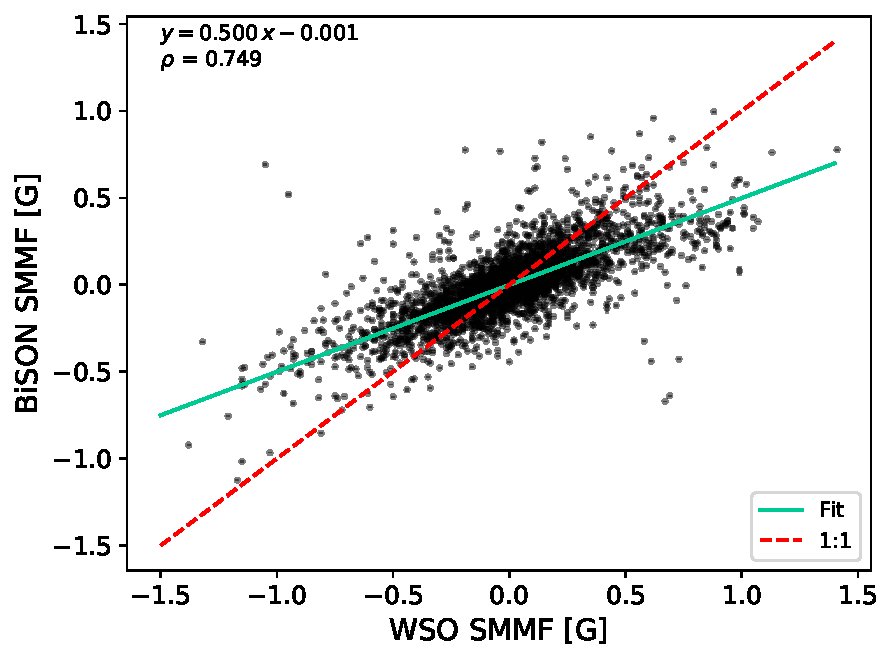
\includegraphics[width=0.47\columnwidth]{BiSON_vs_WSO.pdf}} 
%	\qquad
%	\subfloat[BiSON vs WSO PSDs \label{fig:BiSON_vs_WSO_PSDs}]{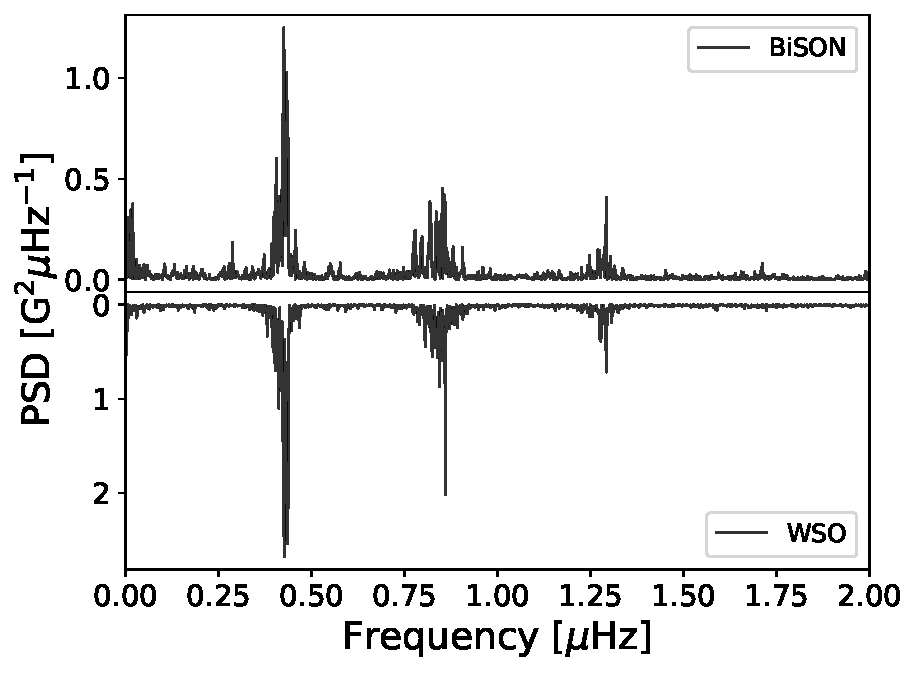
\includegraphics[width=0.47\columnwidth]{BiSON_PSD_vs_WSO_PSD.pdf}}
%	\caption{Comparisons between the BiSON SMMF data and the WSO SMMF data. (a) The correlation between daily-averaged BiSON SMMF and the WSO SMMF. The solid-green line provides the fit to the data, while the dashed-red line shows a 1:1 relation for comparison. (b) Shows a comparison between the power spectra of BiSON and WSO measurements of the SMMF.} \label{fig:BiSON_vs_WSO}
%\end{figure}
%
%%\begin{figure}[ht!]
%%    \centering
%%	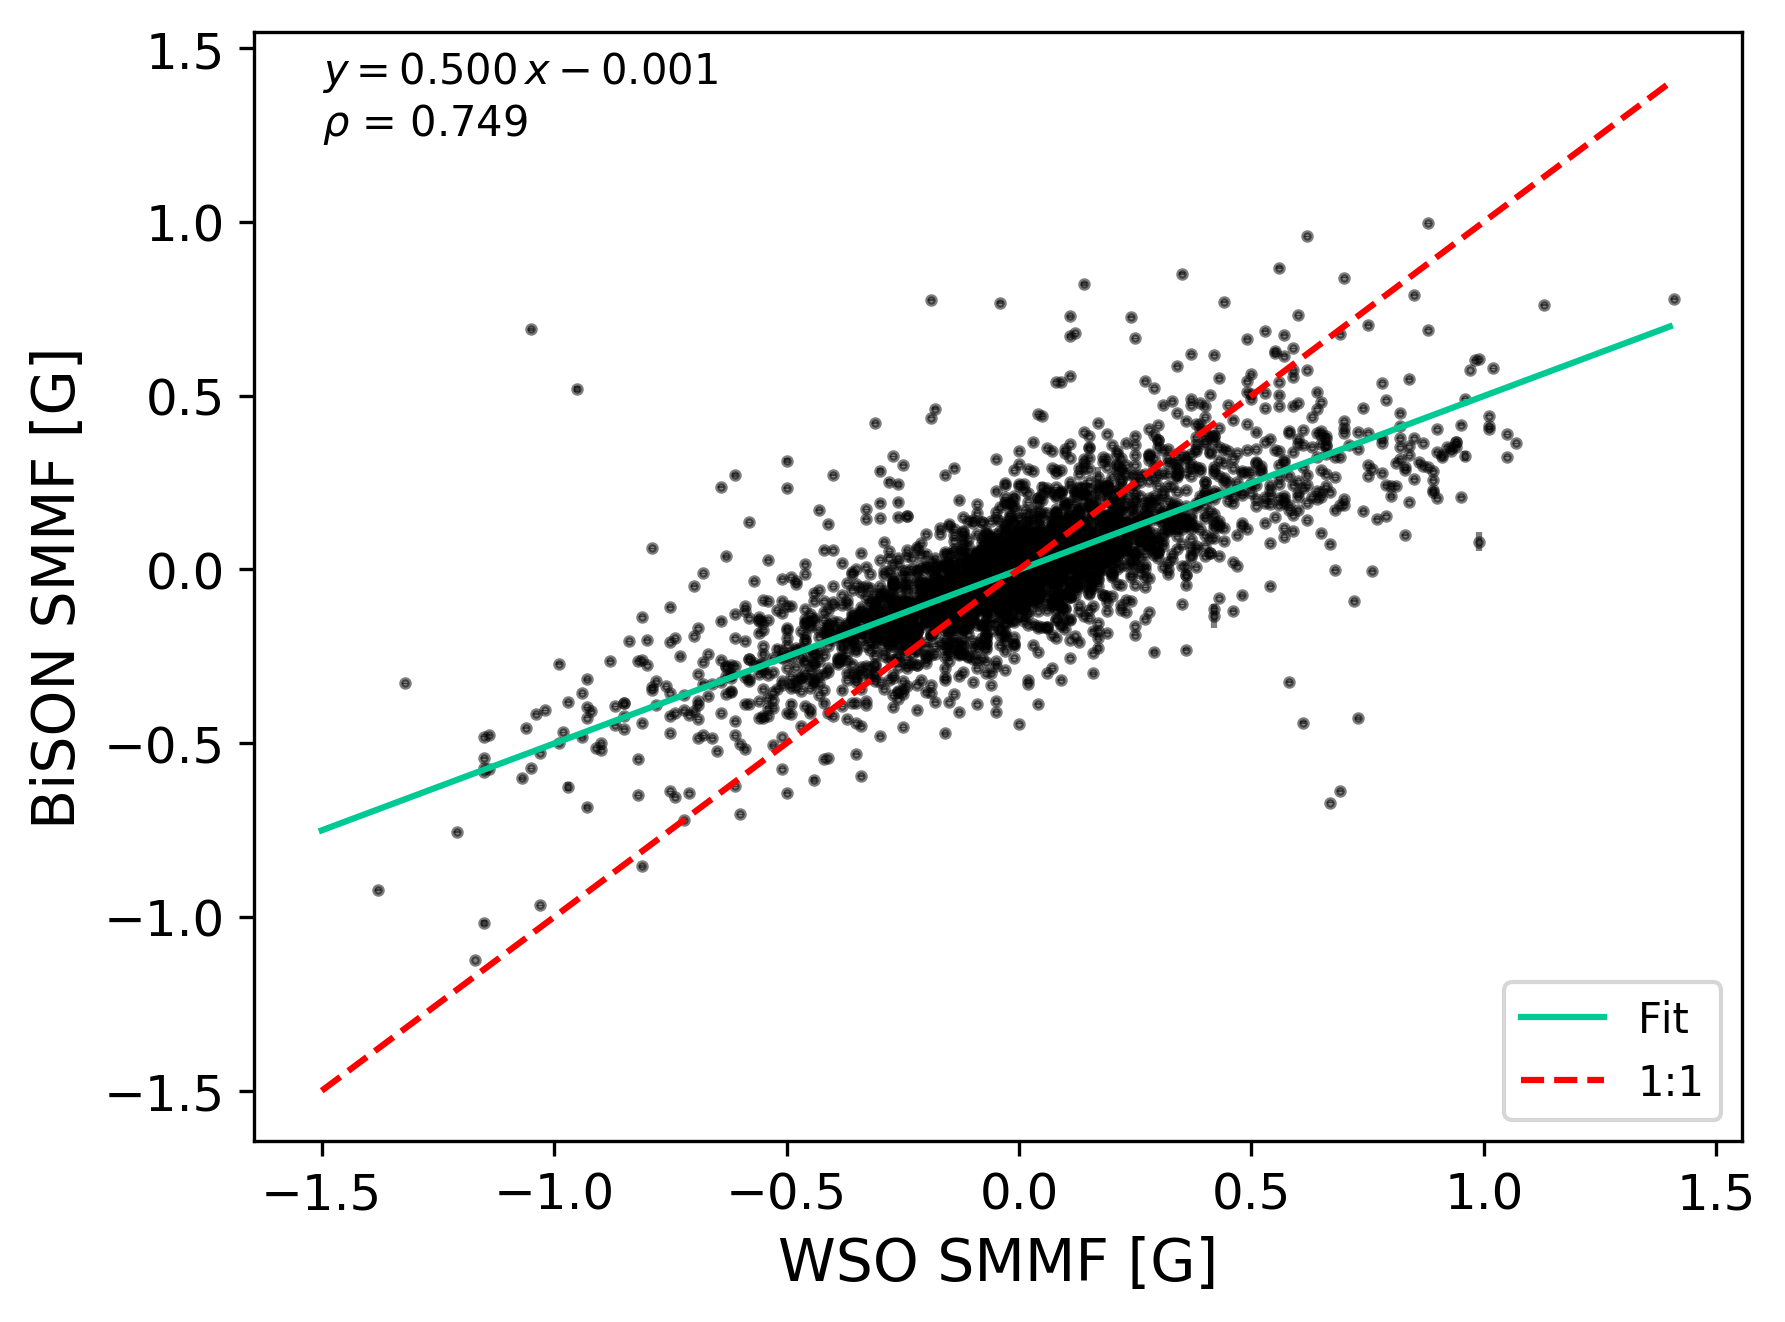
\includegraphics[width=0.75\columnwidth]{BiSON_vs_WSO.png}
%%    \caption{Correlation between the daily SMMF measured by WSO and by the Sutherland BiSON station. }
%%    \label{fig:BiSON_vs_WSO}
%%\end{figure}
%
%
%A possible reason for the differences between the \gls{wso} observations and the \gls{bison} observations may be explained by the formation heights of the lines. Assuming at each level of the solar atmosphere, regions threaded by magnetic field are in pressure equilibrium with those without any field, then the pressure balance can be expressed by equation~(\ref{eq:magnetic_pressure_balance}), where $P_\mathrm{with}$ is the gas pressure in regions with magnetic field, $P_\mathrm{without}$ in those without, and $B^2/2\mu_0$ is the magnetic pressure ($\mu_0$ = magnetic permeability of free space):
%
%\begin{equation}
%P_\mathrm{with} + \frac{B^2}{2\mu_0} = P_\mathrm{without} \, .
%\label{eq:magnetic_pressure_balance}
%\end{equation}
%
%This implies that the observed magnetic field scales like $\sqrt{P}$. Pressure changes exponentially with the scale height, H$_\mathrm{P}$ ($\sim 100-150$ km for the photosphere \citep{christensen-dalsgaard_current_1996}), as described by equation~(\ref{eq:pressure_scale}): 
%
%\begin{equation}
%P_2 = P_1 e^{ - (h_2-h_1)/H_P} \, .
%\label{eq:pressure_scale}
%\end{equation}
%
%Therefore combining both equation~(\ref{eq:magnetic_pressure_balance}) and equation~(\ref{eq:pressure_scale}), we arrive at equation~(\ref{eq:magnetic_scale}):
%
%\begin{equation}
%B_2 = B_1 e^{ - (h_2-h_1)/(2H_P)} \, .
%\label{eq:magnetic_scale}
%\end{equation} 
%
%
%\begin{figure}[ht!]
%	\centering
%	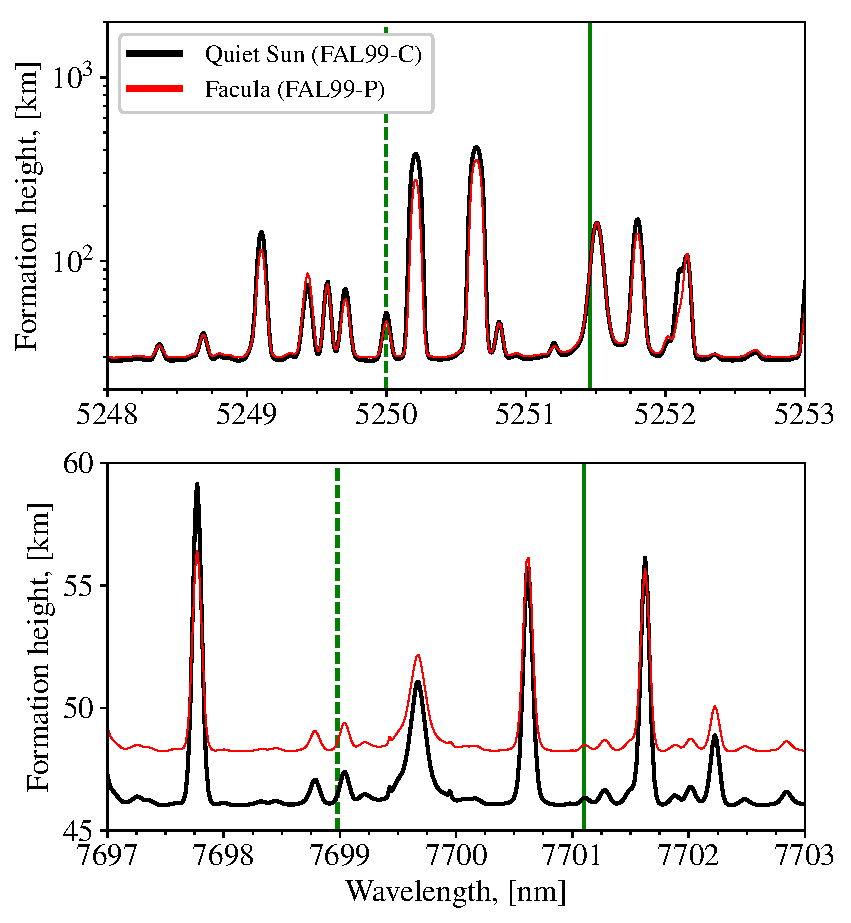
\includegraphics[width=0.85\columnwidth]{fheight_high_res.eps}
%	\caption{Formation heights of emission lines over the wavelength range used for WSO observations (top) and for BiSON observations (bottom). The vertical lines show the wavelengths of the emission lines used for observations in air (dashed) and in vacuum (solid). This plot was provided in private communication courtesy of Rinat Tagirov using the NESSY code.}
%	\label{fig:formation_height}
%\end{figure}
%
%Using a \gls{nlte} simulation to model the spectrum of solar magnetic features (see Figure~\ref{fig:formation_height}, and assuming for some slight calibration issues and Doppler shifting, we might suppose that the formation height of the \gls{bison} line (in vacuum) is around 50~km, and for the \gls{wso} line (in vacuum), around 150~km. This would mean that $B_\mathrm{WSO} \approx 0.6\, B_\mathrm{BiSON} - 0.7 \, B_\mathrm{BiSON}$ which disagrees with our observations and the comparison in Figure~\ref{fig:BiSON_vs_WSO}, but agrees more favourably with \citet{chaplin_studies_2003}.
%
%[Need to decide still how to neatly handle the discrepancy between old paper, this work, and WSO...]
%
%
%Finally, we can see quite clearly that the two power spectra align very closely, as shown in Figure~\ref{fig:BiSON_vs_WSO_PSDs}, and that both spectra appear to display an asymmetric peak shape, with a negative asymmetry. The \gls{wso} power spectrum does also appear to display a lower degree of noise compared to \gls{bison}.






%%%%%%%%%%%%%%%%%%%%%%%%%%%%%%%%%%%%%%%%%%%%%%%%%%%%%%%%%%%%%%%%%%%%%
%%%%%%%%%%%%%%%%%%%%%%%%%%%%%%%%%%%%%%%%%%%%%%%%%%%%%%%%%%%%%%%%%%%%%
\section{Methodology}\label{sec:SMMF_method}


%%%%%%%%%%%%%%%%%%%%%%%%%%%%%%%%%%%%%%%%%%%%%%%%%%%%%%%%%%%%%%%%%%%%%
\subsection{Identifying Features in the SMMF Power Spectrum}

As we have 40-second cadence observations of the \gls{smmf}, we were able to investigate the power spectrum up to a Nyquist frequency of $12500~\upmu\mathrm{Hz}$. There are a number of features within the full power spectrum, shown in Figure~\ref{fig:BiSON_FT_full}.

\begin{figure}[ht!]
	\centering
	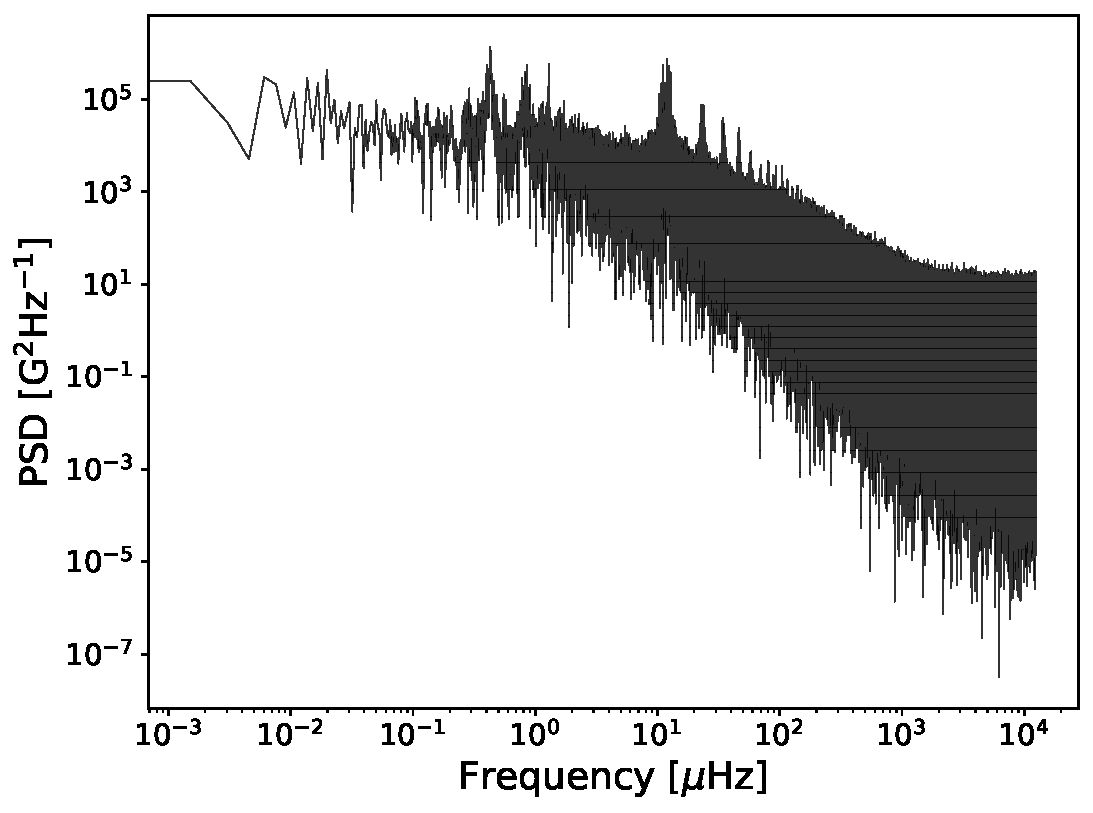
\includegraphics[width=\columnwidth]{BiSON_SMMF_FT_full.pdf}
	\caption{Power spectrum of 40-second cadence SMMF from the Sutherland BiSON station observed between 1992 -- 2012 on a logarithmic scale up to the Nyquist frequency.}
	\label{fig:BiSON_FT_full}
\end{figure}

The peaks between $0.1-2.0~\upmu\mathrm{Hz}$ are a manifestation of a persistent rotational signal in the \gls{smmf}. The distinct set of peaks indicates the existence of a long-lived, inhomogeneous, \gls{rm} source. The \gls{smmf} signal exhibits a quasi-coherent behaviour in the time domain, and based on the comparatively short timescales for the emergence of magnetic features compared to their slow decay (i.e. hours--days compared to weeks--months) \citep{zwaan_solar_1981, harvey_properties_1993, hathaway_sunspot_2008, dacie_evolution_2016}, we assume the evolution of the \gls{rm} component with time is a sudden appearance and a long, exponential decay.

The high Nyquist frequency was critical in uncovering a red-noise-like component in the power spectrum. This component could arise from continuously evolving, short-lived regions of magnetic field linked to magneto-convection, akin to a random walk, which we will dub the \gls{sb} component. Analogous to the \gls{sb}, is the granulation signal observed in the Doppler-velocity measurements of the solar surface \citep{basu_asteroseismic_2017}. It is indeed possible that this is not a real feature in the data and it could also be present due to the high-cadence and low-fill of the observations.

In addition, at low-frequency there is power associated with instrumental noise and solar activity, and at very-high frequency shot-noise is captured which sets the lower limit in power in the spectrum. 

There are also side-band features in the power spectrum at multiples of $1/\mathrm{day}\,\sim\,11.57~\upmu\mathrm{Hz}$. The side-bands are a well-known phenomena in ground-based astronomical observations. They arise from gaps in the data which are a consequence of making single-site, ground-based observations of the Sun.

The duty cycle of the 40--second \gls{bison} observations is very low, at around $\sim$15\%, therefore it was important to take into consideration the effect that gaps in the data have on the power spectrum. Gaps in the data cause an aliasing of power from actual signal frequencies spread to other frequencies in the spectrum, and the nature of the aliasing depends on the properties of the window function of the observations. It is also possible that the \gls{sb} component is an effect of power aliasing due to the low duty cycle of the data. Hence, before modelling the power spectrum, the window function was well-characterised. Through understanding how the duty cycle of the observations affected the power spectrum informed the way we finally parametrised the full model of the power spectrum.


%%%%%%%%%%%%%%%%%%%%%%%%%%%%%%%%%%%%%%%%%%%%%%%%%%%%%%%%%%%%%%%%%%%%%
\subsection{Parametrisation of the SMMF Power Spectrum}

In the frequency domain, each of the \gls{rm} peaks models well as a Lorentzian distribution, similar to peak-bagging modes of solar oscillations \citep{handberg_bayesian_2011, davies_low-frequency_2014}, which is due to the quasi-coherent nature of the source. The exponential decay of the \gls{rm} \gls{smmf} source gives width to the peaks in the power spectrum, which we can measure to infer their lifetime.

A single, symmetric Lorentzian peak can be modelled by:
%
\begin{equation}
L_n(\nu; \Gamma, A_n, \nu_n) = \frac{2{A_n}^2}{\pi \Gamma} \left(1 + \left(\frac{\nu - \nu_{n}}{\Gamma /2}\right)^2\right)^{-1} \, ,
\label{eq:symm_lorentzian}
\end{equation}
%
where $\nu$ is frequency, $A_n$ is the \gls{rms} amplitude of the \gls{rm} component in the time-domain, $\Gamma$ is the linewidth of the \gls{rm} peak, $\nu_n$ is the frequency of the \gls{rm} peak, and $n$ simply flags each peak. The mean-squared power in the time domain from the RM component of the SMMF is given by the sum of the ${A_n}^2$ of the individual harmonics in the power spectrum.

Upon closer inspection of the power spectrum it is possible to see that the peaks appear to exhibit an asymmetric shape (see Fig.~\ref{fig:BiSON_SMMF} and Fig.~\ref{fig:BiSON_FT_full}). Taking inspiration from \citet{howe_solar_2020}, it is possible to allow for asymmetry, which is controlled by the asymmetry parameter, $\alpha$ \citep{stancik_simple_2008}:
%
\begin{equation}
L_n(\nu; \Gamma, A_n, \nu_n) = \frac{2{A_n}^2}{\pi \Gamma(\nu)} \left(1 + \left(2X(\nu)\right)^2\right)^{-1} \, ,
\label{eq:asymm_lorentzian}
\end{equation}
%
where:
%
\begin{equation}
X(\nu) = (\nu - \nu_n)/\Gamma(\nu) \, ;
\label{eq:asymm_freq}
\end{equation}
%
\begin{equation}
\Gamma(\nu) = 2\Gamma / [1 + \exp^{-\alpha(\nu - \nu_n)}] .
\label{eq:asymm_width}
\end{equation}

%This parametrisation of the asymmetric Lorentzian stops any of the power from becoming negative. 
In the limit where $\alpha \rightarrow 0$, we see that $\Gamma(\nu) \rightarrow \Gamma$, thus the asymmetric expression equates to the symmetric expression.

The model function used to describe the \gls{rm} signal in the power spectrum is given by equation~(\ref{eq:lorentzian_fit}); the sum of $N$ Lorentzian-peaks:
%
\begin{equation}
P(\nu) = \sum_{n=1}^{N} L_n(\nu; \Gamma, A_n, \nu_n) \, .
\label{eq:lorentzian_fit}
\end{equation}

The subscript, $n$, describes a single peak in the power spectrum; in implementing the model we constrain the central frequency for each of the peaks such that they must be integer values of $\nu_0$: $\nu_n \, = \, n \nu_0$. This means that we define a single rotation frequency only, and subsequent peaks are harmonics. It is worth noting explicitly that this function assumes the linewidth of each Lorentzian peak is the same; only their amplitudes and central frequencies differ.

When modelling the power spectrum we attempted the fit with both of the symmetric and asymmetric Lorentzian expressions, independently. Firstly we modelled using the symmetric Lorentzian, and subsequently, using the asymmetric Lorentzian. This would determine whether there is a necessity for the addition of the asymmetry parameter.

Through both formulations we can measure the $e$-folding lifetime of the amplitude of the \gls{rm} component ($T_e$), as it is related to the linewidth of the peak by:
%
\begin{equation}
\Gamma  = (\pi \, T_e)^{-1} \, .
\label{eq:mode_lifetime}
\end{equation}


The low-frequency power due to instrumental drifts and solar activity can be reasonably well captured by the inclusion of a zero-frequency centred Lorentzian, i.e. Harvey-function, given by:
%
\begin{equation}
H(\nu; \sigma, \tau) = \frac{4{\sigma}^2\tau}{1 + (2\pi \nu\tau)^2} \, ,
\label{eq:harvey}
\end{equation}
%
where $\sigma$ is the characteristic amplitude of the low frequency signal, and $\tau$ describes the characteristic timescale of the excursions around zero in the time-domain.

%The \gls{sb} component can also be modelled using the Harvey-function, where $\sigma$ is the characteristic amplitude of the red-noise signal and $\tau$ is its characteristic timescale.

Finally, the high frequency power is accounted for by the inclusion of a constant offset due to shot-noise, $c$.


%%%%%%%%%%%%%%%%%%%%%%%%%%%%%%%%%%%%%%%%%%%%%%%%%%%%%%%%%%%%%%%%%%%%%
\subsection{Modelling the SMMF Power Spectrum}
\label{sec:method_modelling}

Parameter estimation was performed in a Bayesian manner using a \gls{mcmc} fitting routine. Following from Bayes’ theorem we can state that the posterior probability distribution, $p({\bf a} | D, I)$, is proportional to the likelihood function, $L(D | {\bf a}, I)$, multiplied by a prior probability distribution, $p({\bf a} | I)$:
%
\begin{equation}
p({\bf a} | D, I) \propto L(D | {\bf a}, I) \, p({\bf a} | I) \, ,
\label{eq:bayes}
\end{equation}
%
where $D$ are the data, and $I$ is any prior information.

To perform the \gls{mcmc} integration over the parameter space we must define a likelihood function; however, in practice, it is more convenient to work with logarithmic probabilities. The noise in the power spectrum is distributed as $\chi^2$ 2 degrees-of-freedom \citep{handberg_bayesian_2011, davies_low-frequency_2014}, therefore the log likelihood function is:
%
\begin{equation}
\ln{(L)} = - \sum\limits_{i} \left\{ \ln{(M_{i}({\bf a}))} + \frac{O_i}{M_{i}({\bf a})} \right\} \, ,
\label{eq:likelihood_functino}
\end{equation}
%
for a model, $M_i$, with parameters, ${\bf a}$, and observed power, $O_i$, where $i$ describes the frequency bin. This likelihood function assumes that all the frequency bins are statistically independent but the effect of the window function means that they are not. We handled this issue by using simulations based on the artificial data discussed in Section~\ref{sec:window_fn}.

%When modelling the power spectrum we used the affine-invariant \gls{mcmc} sampler {\verb emcee } \citep{foreman-mackey_emcee_2013} to explore the posterior parameter space. The chains are not independent within {\verb emcee }, therefore convergence was interrogated using the integrated autocorrelation time, to quantify the effects of sampling error on the results and to ensure we used a sufficient number of effective samples.

The prior information on each of the parameters used during the \gls{mcmc} is discussed below, in Section~\ref{sec:BiSON_reults}.

The affine-invariant \gls{mcmc} sampler {\verb emcee } \citep{foreman-mackey_emcee_2013} was employed to explore the posterior parameter space. The chains are not independent when using {\verb emcee }, therefore convergence was interrogated using the integrated autocorrelation time. We computed the autocorrelation time and found $\tau \sim 120$~steps. \cite{foreman-mackey_emcee_2013} suggests that chains of length $\geq 50\tau$ are often sufficient. After a burn in of 6000 steps, we used 7000 iterations on 50 chains to explore the posterior parameter space, which was sufficient to ensure we had convergence on the posterior probability distribution.

%%%%%%%%%%%%%%%%%%%%%%%%%%%%%%%%%%%%%%%%%%%%%%%%%%%%%%%%%%%%%%%%%%%%%
\subsection{Comparison with the WSO SMMF}

To provide comparative results on the inferences from the \gls{bison} \gls{smmf}, we repeated the analysis on the power spectrum of the \gls{wso} \gls{smmf}. The \gls{wso} data are only provided on a daily cadence, hence the Nyquist frequency is lower than for 40-second \gls{bison} data, at $\sim$5.79~$\upmu\mathrm{Hz}$, and it was not possible to observe the \gls{sb} component. The analysis was therefore also repeated using the daily-averaged \gls{bison} \gls{smmf}, to provide a more direct comparison between \gls{bison} and \gls{wso}.

The same parametrisation as outlined above was relevant to the modelling of the features in the \gls{wso} \gls{psd}, and the \gls{rm} peaks were fitted using a model with symmetric Lorentzian peaks and separately with asymmetric Lorentzian peaks.


%%%%%%%%%%%%%%%%%%%%%%%%%%%%%%%%%%%%%%%%%%%%%%%%%%%%%%%%%%%%%%%%%%%%%
%%%%%%%%%%%%%%%%%%%%%%%%%%%%%%%%%%%%%%%%%%%%%%%%%%%%%%%%%%%%%%%%%%%%%
\section{Results}\label{sec:SMMF_reults}

%%%%%%%%%%%%%%%%%%%%%%%%%%%%%%%%%%%%%%%%%%%%%%%%%%%%%%%%%%%%%%%%%%%%%
\subsection{Investigation of the Window Function}\label{sec:window_fn}


Due to the low fill of data, we see the effects of daily and random gaps on the power spectrum. Periodic gaps in the data give rise to sidebands in the power spectrum and random gaps cause a more broadband shifting of power, meaning that some power from the low-frequency \gls{rm} component in the power spectrum is aliased to higher frequencies. First we will concentrate specifically on the effect of daily, periodic gaps in the data. The daily, periodic gaps in the \gls{bison} data, due to single-site observations, produce sidebands around a frequency of 1/day $\sim$~11.57 $\upmu$Hz and its harmonics.

The frequency (and harmonics) of the \gls{rm} component are located near zero ($\nu_0 \sim \,0.4 \, \upmu\mathrm{Hz}$). We are usually only interested in the real, positive frequencies but due to their close proximity to zero, they are reflected back as a product of the aliasing and hence there are negative and positive side-bands in the (positive frequency) power spectrum. When considering the aliased power, both the positive and negative side-bands must be taken into account. The aliased power is located at frequencies:
%
\begin{equation}
\nu_{n, i} = i \, (\frac{1}{\mathrm{day}} \pm \nu_{n}) \, ,
\label{eq:sidebands}
\end{equation}
%
where $i$ denotes the side-band number, and $n$ denotes the harmonic of the mode.

The side-band structure implied by equation~(\ref{eq:sidebands}) is shown clearly in the \gls{smmf} power spectrum in Figure~\ref{fig:sideband_locations}. It is clear that we could therefore have used the predicted locations of the aliased power and incorporated them into the model for the full power spectrum. This would, however, have required us to explicitly model some $\sim$1100 groups of side-bands in order to cover this effect over the entire frequency range, and each group would have required a unique parameter to control the fraction of power that was contributed to the full \gls{psd}. It would have become computationally expensive to model each aliased peak and there would certainly have been room for degeneracy issues to occur.

\begin{figure}[ht!]
	\centering
	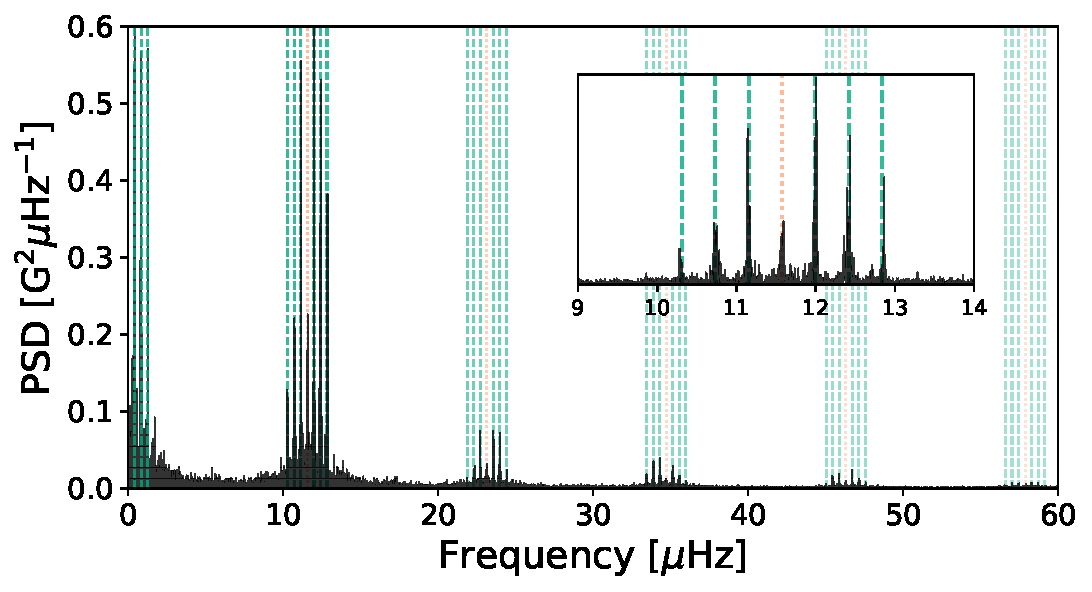
\includegraphics[width=\columnwidth]{sideband.pdf}
	\caption{Locations of aliased power in side-band peaks. The orange, dotted-lines show the locations of frequencies at multiples of 1/day. The green, dashed-lines show the locations of the side-band peaks -- harmonic frequencies reflected around multiples of 1/day.  The inset shows a zoom of one set of side-band peaks around 1/day.}
	\label{fig:sideband_locations}
\end{figure}


A more desirable, and we shall see more accurate, approach was to utilise the power spectrum of the window function itself. This approach not only takes into account the effect of daily, periodic gaps in the data, but also the more complex features that manifest in the power spectrum due to the random gaps in the data. To do this, the Fourier transform of the window function describing the duty cycle of observations was computed (i.e. $\left|\mathcal{F}\left[g(t)\right]\right|^2$), where the duty cycle function, $g(t)$, is given by:
%
\begin{equation}
g(t) = 
\begin{cases} 
1 & \text{for } |B(t)| > 0 \\
0       & \text{for } |B(t)| = 0
\end{cases} \, .
\label{eq:window}
\end{equation}

In Figure~\ref{fig:window_function_PSDs} the power spectrum of the window function is shown. Furthermore, to demonstrate the effect of the window function on the power spectrum, an artificial spectrum was simulated with a single Lorentzian peak, following equation~(\ref{eq:lorentzian_fit}). By computing the inverse Fourier transform, an artificial time-series was generated over the same epoch as the \gls{bison} \gls{smmf} observations. We were then able to examine the effects of injecting gaps into the data that were concurrent with the \gls{bison} \gls{smmf} gaps. 


\begin{figure}[ht!]
	\centering
	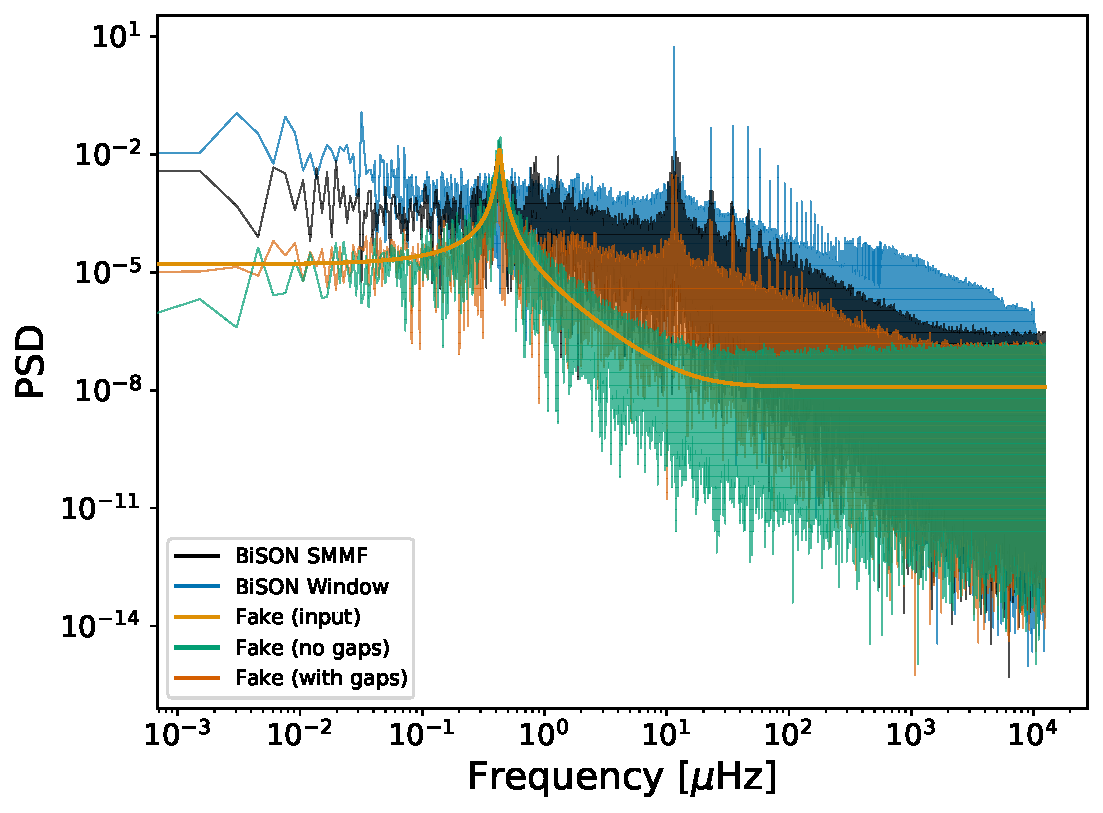
\includegraphics[width=\columnwidth]{gap_test.pdf}
	\caption{The effects of the window function on the power spectrum is shown by using a fake data set and this is compared to the BiSON power spectrum. Black line: BiSON SMMF PSD; blue line: power spectrum of the window function; green and dark-orange lines: the power spectrum of the artificial data without and with gaps, respectively; light orange line: the input peak used to generate the artificial data over-plotted. The power spectra of the BiSON SMMF and the window function have been shifted upwards by a factor of 6 and 30, respectively, for clarity.}
	\label{fig:window_function_PSDs}
\end{figure}


%\begin{figure}[ht!]
%	\centering
%	\subfloat[Black line: BiSON SMMF PSD; blue line: power spectrum of the window function; green and dark-orange lines: the power spectrum of the artificial data without and with gaps, respectively; light orange line: the input peak used to generate the artificial data over-plotted. The lines have been offset for clarity. \label{fig:gap_test_top_plot}]{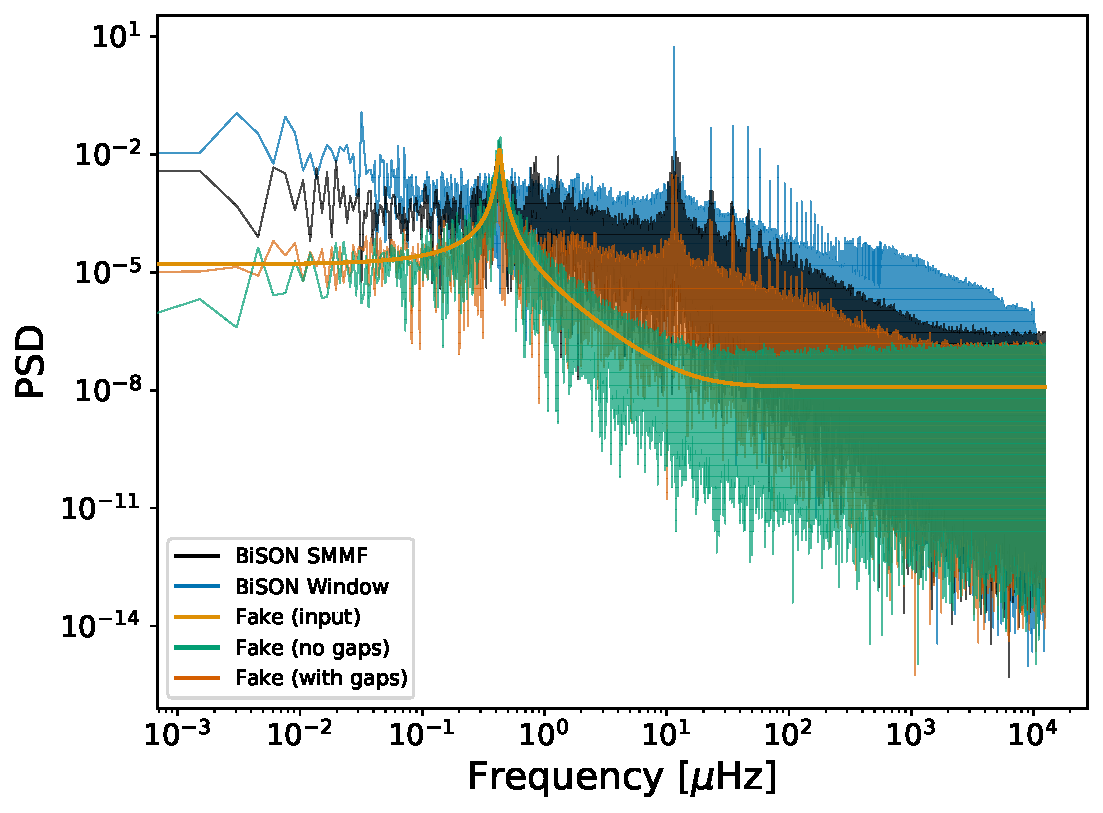
\includegraphics[width=0.7\columnwidth]{gap_test.pdf}}
%	\qquad
%	\subfloat[Dark-orange line: the power spectrum of the artificial data with gaps; solid-grey line: input PSD convolved with the window function; dashed-black line: input PSD convolved with the power spectrum and adjusted for the duty cycle. \label{fig:gap_test_bottom_plot}]{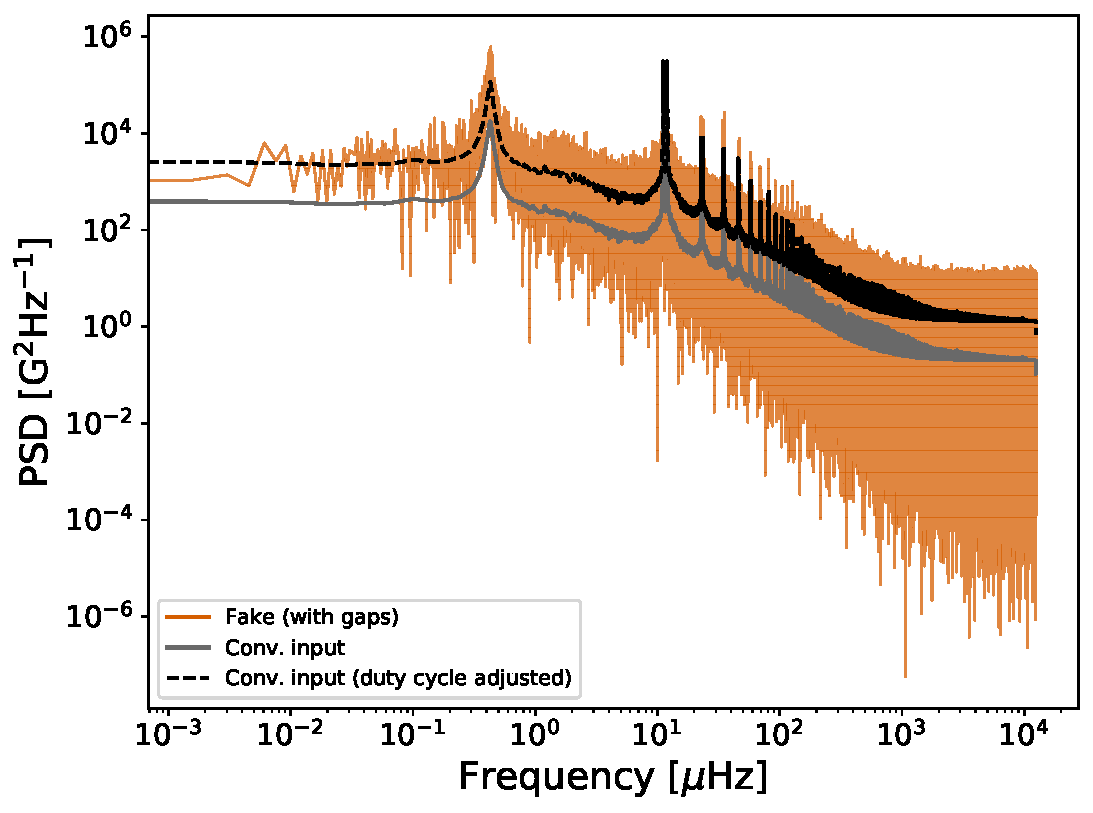
\includegraphics[width=0.7\columnwidth]{gap_test_conv.pdf}}
%	\caption{(a) The effect on the power spectrum due to periodic gaps in the data. (b) The effect of the convolution between the window function and the input power spectrum used to make the fake data, highlighting the need to correctly adjust the power for the duty cycle.}
%	\label{fig:window_function_PSDs}
%\end{figure}
%%top: \label{fig:gap_test_top_plot}
%%bottom: \label{fig:gap_test_bottom_plot}


As well as the power spectrum of the window function, Figure~\ref{fig:window_function_PSDs} also shows the underlying noise-free peak that describes the fake data and the power spectra of the artificial data with and without the injected gaps. The power spectrum of the \gls{bison} \gls{smmf} data is also plotted for comparison.
% Note this comes from: /mnt/storage/003. Data/015. BiSON/SMMF/Fake/Fake_data/1_peak/...

It is strikingly clear from Figure~\ref{fig:window_function_PSDs} that the shape of the spectrum of the window function has a remarkable resemblance to the \gls{bison} \gls{smmf} spectrum and the output of the artificial spectrum with gaps injected. This demonstrates that the periodic window function, with such a low duty cycle, has a significant effect on the power spectrum of the input signal, which not only produces the diurnal sidebands, but also a broadband spread of the power.

Due to the broadband shape of the window function power spectrum compared to the \gls{bison} \gls{smmf}, it appears that there is actually no detectable red-noise-like, \gls{sb} component in the \gls{smmf}; it is instead a manifestation of the periodic gaps in the data. %There is still a necessity for the low-frequency Harvey function in the model (i.e. equation~(\ref{eq:harvey})) to describe the power close to zero, due to instrumental drifts and solar activity.

To analytically understand this effect, we can express the time series of observed data ($y(t)$) as a multiplication of the uninterrupted, underlying signal ($f(t)$) with the window function ($g(t)$), i.e.:
%
\begin{equation}
y(t)  = f(t) \, g(t)
\label{eq:timeseries} \, .
\end{equation}

In the frequency domain, the Fourier transform of a product becomes the convolution of the transformed components. It is possible to express the observed power spectrum of data with periodic gaps in terms of the window function and the gap-free power spectrum, given by:
%
\begin{equation}
P'(\nu; \,{\bf a}) \, = \, P(\nu; \,{\bf a}) * \left|\mathcal{F}\left[g(t)\right]\right|^2 \, .
\label{eq:PSD_fit_conv}
\end{equation}

Therefore to model the observed power spectrum in a robust manner, which takes into account the intricacies caused by gaps in the data, we used a model which was formed of a model power spectrum, $P(\nu; \,{\bf a})$, convolved with the Fourier transform of the window function describing the duty cycle of observations ($\left|\mathcal{F}\left[g(t)\right]\right|^2$), i.e. a model described by equation~(\ref{eq:PSD_fit_conv}), where:
%
\begin{equation}
P(\nu; \,{\bf a}) = \sum_{n=1}^{N} L_n(\nu; \Gamma, A_n, \nu_n) \, + \, H(\nu; \sigma, \tau) \, + \, c \, .
\label{eq:PSD_model}
\end{equation}

Care was taken to ensure Parseval's theorem was obeyed, and no power was lost or gained from the convolution operation: 
%
\begin{equation}
\sum_{\nu} P'(\nu) \, = \,\sum_{\nu} P(\nu) \, = \, \frac{1}{N} \sum_{t}  B(t)^2 \, ,
\label{eq:parseval}
\end{equation}
%
where $N$ here is the number of observed cadences.


%The likelihood of the resulting model from the convolution, $P'(\nu; \,{\bf a})$, was then maximised to give the best fitting parameters.

%We demonstrated the convolution process by performing the convolution between the noiseless peak used to generate the artificial data and the window function. The result of this is shown in Figure~\ref{fig:gap_test_bottom_plot}. Due to method adopted for the convolution, the overall power was reduced as can be seen by the solid-grey line in Figure~\ref{fig:gap_test_bottom_plot}. It was therefore necessary to adjust the resultant power spectrum by the duty cycle factor, i.e. $\sim 15\%$ for \gls{bison} 40-s cadence observations, which produced the dashed-black line in Figure~\ref{fig:gap_test_bottom_plot}, which aligns with the power spectrum of the artificial data with gaps.

%To further demonstrate the effects of the convolution process during the modelling, 
To demonstrate this method, as a proof-of-concept, we fit a model of a single Lorentzian peak, plus a shot-noise background, to the gap-free fake \gls{psd} (without the convolution) and the fake \gls{psd} using the gaps (requiring the convolution). The modelling was performed using the affine-invariant \gls{mcmc} sampler {\verb emcee } \citep{foreman-mackey_emcee_2013} to explore the posterior parameter space, and the results of this fit are summarised in Table~\ref{tab:fake_1pk_params}. 


%\begin{table}[ht!]
%	\begin{center}
%		\caption{Model parameter values for the generation of artificial data, and the median posterior values for the fit to the power spectra generated with and without the gaps in the data. Numbers in brackets denote uncertainties on the last 2 digits, and all uncertainties correspond to the $68 \%$ credible intervals either side of the median.}
%		\label{tab:fake_1pk_params}
%		\begin{tabular}{l c c c r}
%			\hline
%			{\bf Parameter} & {\bf Input} & {\bf Fit (no gaps)} & {\bf Fit (gaps)} & {\bf Unit} \\
%			\hline
%			
%			{$\nu_0$} & {0.42867} & {0.4277$\left(_{-18}^{+18}\right)$} & {0.4261$\left(_{-03}^{+03}\right)$} & {$\mu\mathrm{Hz} $}\\
%			
%			{$\Gamma$} & {0.030} & {0.0279$\left(_{-36}^{+37}\right)$} & {0.0340$\left(_{-06}^{+06}\right)$} & {$\mu\mathrm{Hz} $} \\
%			
%			{$A$} & {100.0} & {101.2$_{-6.0}^{+7.3}$} & {282.56$\pm 0.25$} & {$\mathrm{mG}$} \\
%					
%			{$c$} & {0.20} & {0.1872$\left(_{-03}^{+03}\right)$} & {1.2009$\left(_{-08}^{+08}\right)$} & {$\mathrm{G}^2\mathrm{Hz}^{-1}$} \\	
%			
%			\hline
%		\end{tabular}
%	\end{center}
%\end{table}

\vspace{1em}

\begin{table}[ht!]
	\begin{center}
		\caption{Model parameter values for the generation of artificial data, and the median posterior values for the fit to the power spectra generated with and without the gaps in the data. Numbers in brackets denote uncertainties on the last 2 digits, and all uncertainties correspond to the $68 \%$ credible intervals either side of the median.}
		\label{tab:fake_1pk_params}
		\begin{tabular}{l c c c r}
			\hline
			{\bf Parameter} & {\bf Input} & {\bf Fit (no gaps)} & {\bf Fit (gaps)} & {\bf Unit} \\
			\hline
			
			{$\nu_0$} & {0.42867} & {0.4277$\left(_{-18}^{+18}\right)$} & {0.4261$\left(_{-03}^{+03}\right)$} & {$\upmu\mathrm{Hz} $}\\
			
			{$\Gamma$} & {0.030} & {0.0279$\left(_{-36}^{+37}\right)$} & {0.0340$\left(_{-06}^{+06}\right)$} & {$\upmu\mathrm{Hz} $} \\
			
			{$A$} & {100.0} & {101.2$_{-6.0}^{+7.3}$} & {111.7$\pm 0.1$} & {$\mathrm{mG}$} \\
			
			{$c$} & {0.20} & {0.1872$\left(_{-03}^{+03}\right)$} & {0.1876$\left(_{-01}^{+01}\right)$} & {$\mathrm{G}^2\mathrm{Hz}^{-1}$} \\	
			
			\hline
		\end{tabular}
	\end{center}
\end{table}

%There were several points uncovered about the convolution process in this fitting procedure that we had to take into consideration. Firstly, we found agreement with the effect on the total power observed in Figure~\ref{fig:window_function_PSDs}. The median posterior values of the amplitude and shot noise parameters were affected by the duty cycle, compensating for the effect on the power, which resulted in the amplitude posterior being too large by a factor of the square-root of the duty cycle ($\sim \sqrt{0.15}$) and the shot noise being too large by a factor of the duty cycle ($\sim 0.15$). This again highlights the necessity to incorporate the duty cycle into the convolution to ensure Parseval's theorem is obeyed. After the correction, the median posterior values for the amplitude and noise become: 111.7$\pm0.1$~mG and 0.1876$\left(_{-01}^{+01}\right)$~$\mathrm{G}^2\mathrm{Hz}^{-1}$, respectively, which are in-line with the expected values.

As we can see from the results in Table~\ref{tab:fake_1pk_params}, the median values of the parameter posterior distributions without the gaps are in accordance with the input values, which were used when generating the artificial data, within uncertainties. When the gaps were introduced, the median values of the parameter posterior distributions were close, but the widths of the distributions (which give implied confidence intervals) did not overlap. %We observe that the uncertainties are underestimated in the case using the convolution process.

%In addition, 
Through this demonstration we observed that, as a result of the convolution in the model, the widths of the posterior distributions for the model parameters were systematically underestimated. This effect arises because we do not account explicitly for the impact of the window function convolution on the covariance of the data. To perform the full likelihood evaluation, with the correlated noise, requires large-data computational linear algebra (i.e. the inversion of an N-by-N diagonal-constant/Toeplitz matrix, where N is the size of data); unfortunately the process of fully accounting for the correlated noise in this scenario was too computationally expensive, due to the large data set with $\sim10^7$ data points. Our ability to resolve the model parameters is well represented in the case where the convolution was not performed; this helped us to understand how the convolution affected our ability to measure the true posterior widths, which allowed us to account for the systematic underestimate of the credible regions of the posterior distributions. We assumed the for $\nu_0$ and $c$, we have an accuracy of $\sim$0.5\% each; for $\Gamma$, an accuracy of $\sim$15\%; for $A$, an accuracy of $\sim$10\%. Using these uncertainty estimates, the parameter posterior distributions for the convolution model are in accordance with the input values.

When modelling the power spectrum of the observed \gls{bison} \gls{smmf}, these factors allowed us to account for the systematic underestimate of the posterior widths from the convolution.

%From this exercise we learned that during the modelling of the \gls{bison} (and \gls{wso}) power spectra, we needed to account for the duty cycle to ensure no loss of power from the convolution process. We have also learnt that the likelihood evaluation does not properly take into consideration the effect of the correlated noise in the power spectrum, but it is too computationally expensive to account for.



%%%%%%%%%%%%%%%%%%%%%%%%%%%%%%%%%%%%%%%%%%%%%%%%%%%%%%%%%%%%%%%%%%%%%
\subsection{Modelling the BiSON Power Spectrum}\label{sec:BiSON_reults}

As there were many data points in the power spectrum, each likelihood calculation was computationally expensive. In order to reduce the required computation, the \gls{bison} power spectrum was cut at a frequency of 7000 $\upmu\mathrm{Hz}$, as at very high frequency, the spectrum purely represents the shot noise in the \gls{smmf}, and it was deemed as a sufficient limit to still fully converge on the shot noise parameter.

%We have shown the likelihood evaluation does not fully take into account the correlated noise due to the convolution, and doing so would have been too expensive to compute; hence, the pragmatic approach was to ignore the effect of the correlated noise in the convolution on the likelihood calculation.

The \gls{bison} power spectrum was modelled against equation~(\ref{eq:PSD_fit_conv}) (which used equation~(\ref{eq:PSD_model}) with $N = 4$ peaks), for both the symmetric and asymmetric Lorentzian models, using the affine-invariant \gls{mcmc} sampler {\verb emcee } \citep{foreman-mackey_emcee_2013} to explore the posterior parameter space. In the modelling we used uniform prior information, providing reasonable boundaries on each parameter, as detailed below.


\begin{gather*}
%
\nu_0 \, \sim \,\mathcal{U}(0.38, 0.50) \> \upmu\mathrm{Hz} \\
%
\Gamma \, \sim \,\mathcal{U}(0.00, 0.11)  \> \upmu\mathrm{Hz} \\
%
A_1 \, \sim \,\mathcal{U}(100, 350)  \> \mathrm{mG} \\
%
A_2 \, \sim \,\mathcal{U}(50, 200)  \> \mathrm{mG} \\
%
A_3 \, \sim \,\mathcal{U}(20, 150)  \> \mathrm{mG} \\
%
A_4 \, \sim \,\mathcal{U}(10, 100)  \> \mathrm{mG} \\
%
\sigma \, \sim \,\mathcal{U}(0.01, 500)  \> \mathrm{mG} \\
%
\tau \, \sim \,\mathcal{U}(0.10, 200)  \> 10^6 \, \mathrm{s} \\
%
c \, \sim \,\mathcal{U}(10^{-3}, 10^{2})  \> \mathrm{G}^2 \, \mathrm{Hz}^{-1} \\
%
\alpha \, \sim \,\mathcal{U}(-500, 0)\\
\end{gather*}


In Table~\ref{tab:PSD_fit_params} the median values of adjusted, marginalised posterior distributions for each of the model parameters are displayed, for both the symmetric and asymmetric models. The resultant posterior distributions were approximately normally distributed and there was no significant covariance between parameters, therefore uncertainties on the parameters correspond to the $68 \%$ credible intervals either side of the median. We note the we have previously shown the convolution results in a systematic underestimate in the width of the posterior distributions and thus here we are presenting an estimation of the true uncertainties based on multiplying by the factors acquired from the artificial simulations in Section~\ref{sec:window_fn}.

%%\begin{table}[ht!]
%%	\begin{center}
%%		\caption{Median values of the marginalised posterior distributions for each model parameter in the fit to the BiSON power spectrum. Numbers in brackets denote uncertainties on the last 2 digits, and all uncertainties correspond to the $68 \%$ credible intervals either side of the median in the adjusted posteriors.}
%%		\label{tab:PSD_fit_params}
%%		\begin{tabular}{l c c r}
%%			\hline
%%			{\bf Parameter} & {\bf 40-s symm.} & {\bf 40-s asymm.} & {\bf Unit} \\
%%			\hline
%%			
%%			{$\nu_0$} & {0.42699$\left(_{-13}^{+13}\right)$} & {0.42778$\left(_{-14}^{+14}\right)$} & {$\mu\mathrm{Hz} $}\\
%%			
%%			{$\Gamma$} & {0.02639$\left(_{-48}^{+49}\right)$} & {0.03163$\left(_{-71}^{+71}\right)$} & {$\mu\mathrm{Hz} $} \\
%%			
%%			{$A_1$} & {166.0$\pm 2.0$} & {178.9$\pm 1.2$} & {$\mathrm{mG}$} \\
%%			
%%			{$A_2$} & {115.9$\pm 2.3$} & {129.0$\pm 1.2$} & {$\mathrm{mG}$} \\
%%			
%%			{$A_3$} & {83.2$\pm 2.7$} & {93.5$\pm 1.2$} & {$\mathrm{mG}$} \\
%%			
%%			{$A_4$} & {32.6$\pm 4.3$} & {38.9$\pm 1.9$} &  {$\mathrm{mG}$} \\	
%%			
%%			{$\tau$} & {51.8$_{-3.7}^{+3.9}$} & {62.7$_{-4.6}^{+4.9}$} & {$\mathrm{days}$} \\	
%%			
%%			{$\sigma$} & {83.4$\pm 3.5$} & {79.1$\pm 1.4$} &  {$\mathrm{mG}$} \\	
%%			
%%			{$c$} & {0.2103$\left(_{-09}^{+09}\right)$} & {0.2102$\left(_{-01}^{+01}\right)$}  & {$\mathrm{G}^2 \, \mathrm{Hz}^{-1}$} \\	
%%			
%%			{$\alpha$} & {--} & {-119.8$_{-7.9}^{+8.0}$} & {--} \\	
%%			\hline
%%		\end{tabular}
%%	\end{center}
%%\end{table}

\vspace{1em}

\begin{table}[ht!]
	\begin{center}
		\caption{Median values of the marginalised posterior distributions for each model parameter in the fit to the BiSON power spectrum using symmetric and asymmetric Lorentzian profiles. Numbers in brackets denote uncertainties on the last 2 digits, and all uncertainties correspond to the $68 \%$ credible intervals either side of the median in the adjusted posteriors. The last row in the table shows the Bayesian Information Criterion (BIC) value for each model.}
		\label{tab:PSD_fit_params}
		\begin{tabular}{l c c r}
			\hline
			{\bf Parameter} & {\bf 40-s symm.} & {\bf 40-s asymm.} & {\bf Unit} \\
			\hline
			
			{$\nu_0$} & {0.4270$\left(_{-18}^{+18}\right)$} & {0.4278$\left(_{-18}^{+18}\right)$} & {$\upmu\mathrm{Hz} $}\\
			
			{$\Gamma$} & {0.0264$\left(_{-35}^{+35}\right)$} & {0.0316$\left(_{-41}^{+41}\right)$} & {$\upmu\mathrm{Hz} $} \\
			
			{$A_1$} & {166.0$\pm10.7 $} & {178.9$\pm 11.5$} & {$\mathrm{mG}$} \\
			
			{$A_2$} & {115.9$\pm7.4$} & {129.0$\pm 8.3$} & {$\mathrm{mG}$} \\
			
			{$A_3$} & {83.2$\pm5.3$} & {93.5$\pm 6.0$} & {$\mathrm{mG}$} \\
			
			{$A_4$} & {32.6$\pm2.1$} & {38.9$\pm 2.5$} &  {$\mathrm{mG}$} \\	
			
			{$\tau$} & {51.8$\pm6.8$} & {62.7$\pm8.2$} & {$\mathrm{days}$} \\	
			
			{$\sigma$} & {83.4$\pm5.4$} & {79.1$\pm5.1$} &  {$\mathrm{mG}$} \\	
			
			{$c$} & {0.2103$\left(_{-03}^{+03}\right)$} & {0.2102$\left(_{-03}^{+03}\right)$}  & {$\mathrm{G}^2 \, \mathrm{Hz}^{-1}$} \\	
			
			{$\alpha$} & {--} & {-119.8$\pm15.7$} & {--} \\	
			\hline
			{\bf BIC} & {106} & {122} & {--} \\
			\hline
		\end{tabular}
	\end{center}
\end{table}

%As the asymmetry parameter converged reasonably within the prior bounds, we could deduce that the extra parameter was necessary; the model utilising asymmetric Lorentzian peaks was a better fit to the data than the model with symmetric Lorentzian peaks. However, we also 
We calculated the \gls{bic} to aid our model selection, to determine whether the asymmetry was truly necessary or a case of over-fitting to the data. The \gls{bic} for both the symmetric and asymmetric models were $\sim$106 and $\sim$122, respectively. This highlighted that the model using the symmetric Lorentzian profiles was favoured, due to the lower \gls{bic} value. 

The convolved model of the data, using symmetric Lorentzian peaks, is shown in Figure~\ref{fig:BiSON_PSD_fit}, over-plotted on top of the \gls{bison} \gls{smmf} power spectrum.


\begin{figure}[ht!]
	\centering
	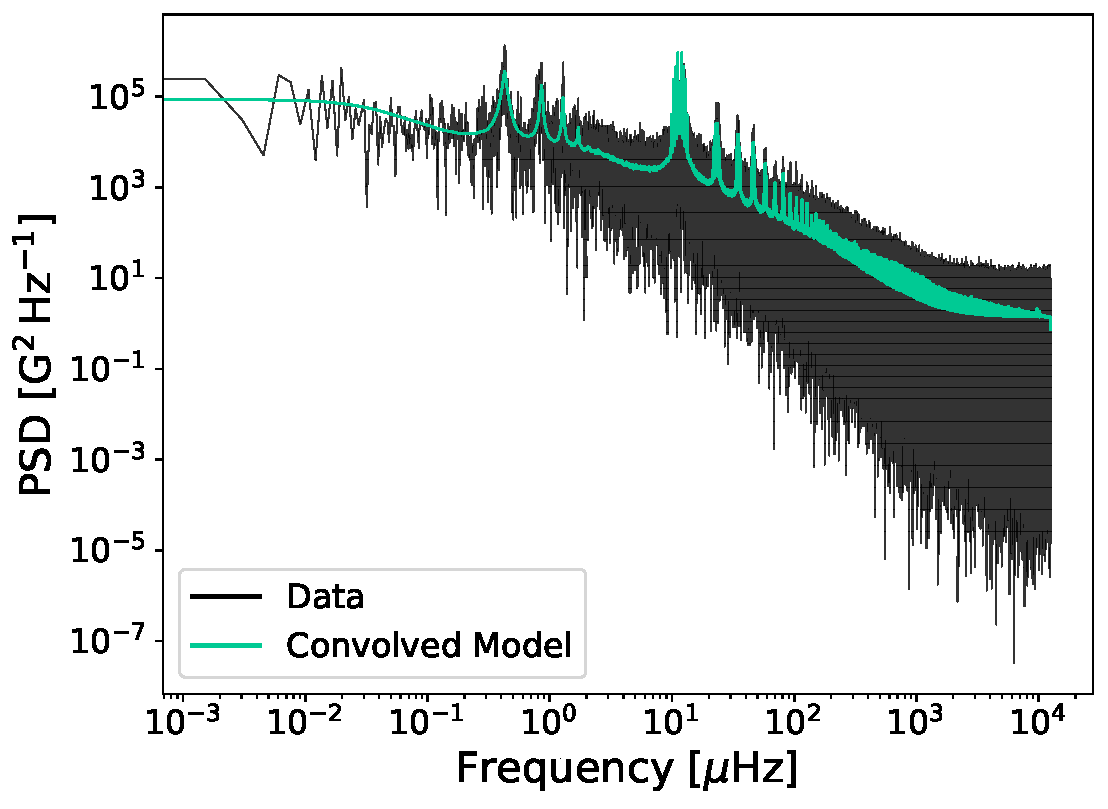
\includegraphics[width=\columnwidth]{BiSON_PSD_model.pdf}
	\caption{Full, modelled power spectrum of the BiSON SMMF on logarithmic axes. The data are displayed in black and the convolved model using symmetric Lorentzian peaks is shown in green.}
	\label{fig:BiSON_PSD_fit}
\end{figure}


The central frequency of this model, $\nu_0$, implies a synodic rotation period of $27.11\pm0.11$~days, and hence a sidereal rotation period of $25.23\pm0.11$~days. The rotation period measured is in agreement with other literature values for the rotation signal in the \gls{smmf} \citep{chaplin_studies_2003, xie_temporal_2017}, and is in accordance with that typically observed for \glspl{ar} and sunspots.

According to the model for differential rotation given by \citet{snodgrass_magnetic_1983} and \citet{brown_inferring_1989}, the measured rotation period implies the \gls{rm} component of the \gls{smmf} is sensitive to a time-averaged latitude at around $12^{\circ}$. This latitude is consistent with those spanned by sunspots and \glspl{ar} over the solar activity cycle \citep{maunder_note_1904, mcintosh_deciphering_2014}, and particularly during the declining phase of the solar cycle \citep{thomas_asteroseismic_2019}. This strongly implies that the origin of the \gls{rm} component of the \gls{smmf} is linked to \glspl{ar} and \glspl{mfc}.

Furthermore, from the measured linewidth of the Lorentzian peaks, we have calculated the lifetime of the \gls{rm} component using equation~(\ref{eq:mode_lifetime}). The linewidth suggests a lifetime of $139.6 \pm 18.5$~days, which is in the region of $\sim 20\pm3$~weeks. The typical lifetime of \glspl{ar} and sunspots is usually on the order of weeks to months, dependent on their size \citep{zwaan_solar_1981, schrijver_photospheric_1994, howard_sunspot_2001, hathaway_sunspot_2008, van_driel-gesztelyi_evolution_2015}, therefore we have measured a lifetime of the \gls{rm} component which is consistent with the lifetime of \glspl{ar} and sunspots. This again suggests that the source of the signal is linked to active regions of magnetic field or similar \glspl{mfc}.

Taking into account the work performed by \citet{bose_variability_2018}, which showed evidence to suggest sunspots did not contribute to the \gls{smmf}, and also our concerns with their methodology, we are cautious to specify that sunspots are the source of the \gls{rm} component; however, this can still not be ruled out altogether. The method of identifying \glspl{ar} or strong \glspl{mfc} in magnetograms by \citet{bose_variability_2018} potentially mis-identified regions of magnetic flux associated with \glspl{ar} and \glspl{mfc} as background flux and it is possible that they do contribute to the \gls{smmf}. By comparison with the work carried out by \citet{kutsenko_contribution_2017}, the work performed in this project agrees that the \gls{smmf} is dominated by features with properties in-line with spots, \glspl{ar}, and \glspl{mfc}, i.e. long-lived and making up a small fraction of the solar disc, confined to active bands of latitude.

With all this considered, we conclude that our investigation of the \gls{bison} \gls{smmf} indicates the \gls{smmf} has its origin in the vicinity of \glspl{ar} and other concentrations of strong flux that are long-lived on the solar disc and exist in active latitudes. Whether or not specifically this is due to spots or other \glspl{mfc} will require further work on the magnetogram thresholding techniques investigating the \gls{smmf}.


%%%%%%%%%%%%%%%%%%%%%%%%%%%%%%%%%%%%%%%%%%%%%%%%%%%%%%%%%%%%%%%%%%%%%
\subsection{Comparison to the WSO Power Spectrum}\label{sec:WSO_reults}

Here we present the results from modelling the \gls{wso} power spectrum; we also show the results of modelling the power spectrum of the daily-averaged \gls{bison} spectrum, to provide a direct comparison between both observations on the same cadence. 

The fill of the \gls{wso} observations over the same epoch as \gls{bison} observations was $\sim 78\%$, and at $\sim 55\%$ for the daily-averaged \gls{bison} observations. As the fill of the daily-averaged \gls{bison} data was higher than the 40-cadence data, the effect of the window function was less prominent. Nevertheless, the power spectra for both daily \gls{wso} and \gls{bison} data were modelled using the convolution approach, as per the previous section. As, compared to the duty cycle of 40-cadence data, the fill is closer to $100\%$, we also expect the effect of the convolution to be less significant on the widths of the posterior distributions for each parameter, and thus the uncertainties to be more representative.

In addition, we also had to account for the sinc-function attenuation effect and reflections of power around the Nyquist frequency, due to the lower Nyquist frequency and its close proximity to the frequencies of the rotation peaks \citep{basu_asteroseismic_2017}.

%The \gls{wso} PSD was modelled using equation~\ref{eq:WSO_PSD_model}, with $N=3$, and $I=2$
%
%\begin{equation}
%P(\nu; \,{\bf a}) = \sum_{n=1}^{N} L_n(\nu; \Gamma, A_n, \nu_n) \, + \, \sum_{i=1}^{I} H_i(\nu; \sigma_i, \tau_i) \, + \, c \, .
%\label{eq:WSO_PSD_model}
%\end{equation}

The daily-averaged \gls{bison} power spectrum was modelled against equation~(\ref{eq:PSD_fit_conv}) using equation~(\ref{eq:PSD_model}) with $N = 4$ peaks, and similarly for the \gls{wso} power spectrum but with $N = 3$ peaks, as a fourth peak was less pronounced. Both fitting routines used the affine-invariant \gls{mcmc} sampler {\verb emcee }  \citep{foreman-mackey_emcee_2013} to explore the posterior parameter space, using 10000 iterations on 50 chains. The convergence was again interrogated using the integrated autocorrelation time, to ensure a sufficient number of effective samples were used; hence ensuring that the posterior distribution was sampled.

In Table~\ref{tab:WSO_SMMF_fit_params} the median values of marginalised posterior distributions for the model parameters are displayed, for both daily \gls{wso} and \gls{bison} data. Reported uncertainties on the parameters correspond to the $68 \%$ credible intervals either side of the median. The systematic underestimate of the posterior width is much less of a concern with these results due to the higher duty cycle; the uncertainties are on the same order as the results not using a convolved model in Table~\ref{tab:fake_1pk_params}. The convolved model for both the \gls{wso} and \gls{bison} data, using symmetric Lorentzian peaks, are shown in Figure~\ref{fig:WSO_and_24h_BiSON_PSD_fit} over-plotted on top their respective \gls{smmf} power spectra.

%\begin{table}[ht!]
%	\begin{center}
%		\caption{Median values of the marginalised posterior distributions for each model parameter in the fit to the WSO power spectrum, adjusted for the duty cycle factor ($\sim 0.778$) in the convolution process. Numbers in brackets denote uncertainties on the last 2 digits, and all uncertainties correspond to the $68 \%$ credible intervals either side of the median.}\label{tab:WSO_SMMF_fit_params}
%		\begin{tabular}{l c c c c r}
%			\hline
%			{\bf Parameter} & {\bf 24-hr symm.} & {\bf 24-hr asymm.} & {\bf Unit} \\
%			\hline
%			
%			{$\nu_0$} & {0.4273$\left(_{-05}^{+05}\right)$} & {0.4290$\left(_{-05}^{+04}\right)$} & {$\mu\mathrm{Hz} $}\\
%			
%			{$\Gamma$} & {0.0209$\left(_{-15}^{+16}\right)$} & {0.0210$\left(_{-15}^{+16}\right)$} & {$\mathrm{mG}$} \\
%			
%			{$A_1$} & {134.4$_{-3.3}^{+3.2}$} & {137.0$_{-3.5}^{+3.4}$} & {$\mathrm{mG}$} \\
%			
%			{$A_2$} & {120.7$\pm 3.4$} & {124.8$_{-3.6}^{+3.5}$} & {$\mathrm{mG}$} \\
%			
%			{$A_3$} & {73.7$\pm 3.5$} & {77.4$\pm 3.8$} & {$\mathrm{mG}$} \\
%			
%			{$\tau$} & {22.5$_{-6.9}^{+10.1}$} & {23.7$_{-7.3}^{+11.1}$} & {$10^6 \mathrm{s}$} \\	
%			
%			{$\sigma$} & {52.1$_{-4.4}^{+4.7}$} & {51.5$_{-4.5}^{+4.6}$} & {$\mathrm{mG}$} \\	
%			
%			{$c$} & {11.4$_{-8.5}^{+17.8}$} & {12.0$_{-8.9}^{+18.6}$} & {$\mathrm{G}^2\mathrm{Hz}^{-1}$} \\	
%			
%			{$\alpha$} & {--} & {-61.7$_{-15.3}^{+13.3}$} & {--} \\	
%			\hline
%		\end{tabular}
%	\end{center}
%\end{table}

%\begin{table}[ht!]
%	\begin{center}
%		\caption{Median values of the marginalised posterior distributions for each model parameter in the fit to the WSO power spectrum, adjusted for the duty cycle factor ($\sim 0.778$) in the convolution process. Numbers in brackets denote uncertainties on the last 2 digits, and all uncertainties correspond to the $68 \%$ credible intervals either side of the median.}\label{tab:WSO_SMMF_fit_params}
%		\begin{tabular}{l c c | c c r}
%			\hline
%			{\bf } & \multicolumn{2}{c |}{\bf WSO} & \multicolumn{2}{c}{\bf BiSON 24-hr} & {\bf } \\
%			{\bf Parameter} & {\bf Symm.} & {\bf Asymm.} & {\bf Symm.} & {\bf Asymm.} & {\bf Unit} \\
%			\hline
%			
%			{$\nu_0$} & {0.4273$\left(_{-05}^{+05}\right)$} & {0.4290$\left(_{-05}^{+04}\right)$} & {0.4244$\left(_{-09}^{+09}\right)$} & {0.4268$\left(_{-09}^{+09}\right)$} & {$\mu\mathrm{Hz} $}\\
%			
%			{$\Gamma$} & {0.0209$\left(_{-15}^{+16}\right)$} & {0.0210$\left(_{-15}^{+16}\right)$} & {0.0400$\left(_{-36}^{+38}\right)$} & {0.0468$\left(_{-36}^{+38}\right)$} & {$\mu\mathrm{Hz} $} \\
%			
%			{$A_1$} & {134.4$_{-3.3}^{+3.2}$} & {137.0$_{-3.5}^{+3.4}$} & {117.8$_{-3.9}^{+4.3}$} & {126.9$_{-4.9}^{+5.3}$} & {$\mathrm{mG}$} \\
%			
%			{$A_2$} & {120.7$\pm 3.4$} & {124.8$_{-3.6}^{+3.5}$} & {106.5$_{-3.8}^{+3.7}$} & {113.6$_{-4.6}^{+4.5}$} & {$\mathrm{mG}$} \\
%			
%			{$A_3$} & {73.7$\pm 3.5$} & {77.4$\pm 3.8$} & {63.1$_{-3.4}^{+3.5}$} & {70.4$_{-3.9}^{+4.2}$} & {$\mathrm{mG}$} \\
%			
%			{$A_4$} & {--} & {--} & {27.4$_{-3.1}^{+3.2}$} & {31.5$_{-3.5}^{+3.6}$} & {$\mathrm{mG}$} \\
%			
%			{$\tau$} & {22.5$_{-6.9}^{+10.1}$} & {23.7$_{-7.3}^{+11.1}$} & {4.4$_{-1.1}^{+1.6}$} & {8.0$_{-2.3}^{+3.5}$} & {$10^6 \mathrm{s}$} \\	
%			
%			{$\sigma$} & {52.1$_{-4.4}^{+4.7}$} & {51.5$_{-4.5}^{+4.6}$} & {80.2$\pm 5.0$} & {75.0$_{-5.7}^{+5.8}$} & {$\mathrm{mG}$} \\	
%			
%			{$c$} & {11.4$_{-8.5}^{+17.8}$} & {12.0$_{-8.9}^{+18.6}$} & {30.6$_{-19.4}^{+17.3}$} & {28.6$_{-18.9}^{+17.9}$} & {$\mathrm{G}^2 \, \mathrm{Hz}^{-1}$} \\	
%			
%			{$\alpha$} & {--} & {-61.7$_{-15.3}^{+13.3}$} & {--} & {-45.8$_{-13.5}^{+12.0}$} & {--} \\	
%			\hline
%		\end{tabular}
%	\end{center}
%\end{table}

\vspace{1em}

% NEW RESULTS AFTER THE APODISATION ETC.
\begin{table}[ht!]
	\begin{center}
		\caption{Median values of the marginalised posterior distributions for each model parameter in the fit to the daily WSO and BiSON power spectra. Numbers in brackets denote uncertainties on the last 2 digits, and all uncertainties correspond to the $68 \%$ credible intervals either side of the median. The last row in the table shows the BIC value for each model.}\label{tab:WSO_SMMF_fit_params}
		\begin{tabular}{l c c | c c r}
			\hline
			{\bf } & \multicolumn{2}{c |}{\bf WSO} & \multicolumn{2}{c}{\bf BiSON 24-hr} & {\bf } \\
			{\bf Parameter} & {\bf Symm.} & {\bf Asymm.} & {\bf Symm.} & {\bf Asymm.} & {\bf Unit} \\
			\hline
			
			{$\nu_0$} & {0.4272$\left(_{-05}^{+05}\right)$} & {0.4290$\left(_{-04}^{+04}\right)$} & {0.4246$\left(_{-09}^{+08}\right)$} & {0.4270$\left(_{-08}^{+08}\right)$} & {$\upmu\mathrm{Hz} $}\\
			
			{$\Gamma$} & {0.0210$\left(_{-15}^{+16}\right)$} & {0.0210$\left(_{-15}^{+16}\right)$} & {0.0359$\left(_{-26}^{+27}\right)$} & {0.0365$\left(_{-29}^{+30}\right)$} & {$\upmu\mathrm{Hz} $} \\
			
			{$A_1$} & {134.8$_{-3.2}^{+3.1}$} & {137.3$\pm 3.5$} & {118.9$_{-3.8}^{+4.2}$} & {125.6$_{-4.4}^{+5.0}$} & {$\mathrm{mG}$} \\
			
			{$A_2$} & {121.6$\pm 3.4$} & {125.9$_{-3.6}^{+3.7}$} & {109.2$_{-3.8}^{+3.6}$} & {115.4$_{-4.4}^{+4.2}$} & {$\mathrm{mG}$} \\
			
			{$A_3$} & {75.1$_{-3.4}^{+3.5}$} & {78.9$_{-3.9}^{+4.0}$} & {64.6$_{-3.5}^{+3.7}$} & {70.1$_{-4.0}^{+4.2}$} & {$\mathrm{mG}$} \\
			
			{$A_4$} & {--} & {--} & {28.0$_{-3.3}^{+3.4}$} & {30.7$_{-3.6}^{+3.7}$} & {$\mathrm{mG}$} \\

%			{$\tau$} & {22.8$_{-7.2}^{+10.5}$} & {23.4$_{-7.3}^{+11.1}$} & {4.3$_{-1.1}^{+1.6}$} & {6.7$_{-1.9}^{+2.8}$} & {$10^6 \mathrm{s}$} \\
			
			{$\tau$} & {263.9$_{-83.3}^{+121.5}$} & {270.8$_{-84.5}^{+128.5}$} & {49.8$_{-12.7}^{+18.5}$} & {77.5$_{-22.0}^{+32.4}$} & {days} \\	
			
			{$\sigma$} & {52.3$\pm 4.6$} & {51.3$_{-4.5}^{+4.6}$} & {81.5$_{-1.1}^{+5.1}$} & {77.1$_{-5.5}^{+5.7}$} & {$\mathrm{mG}$} \\	
			
			{$c$} & {11.7$_{-8.8}^{+18.7}$} & {11.0$_{-8.4}^{+18.4}$} & {0.210$\pm 0.011$} & {0.210$\pm 0.011$} & {$\mathrm{G}^2 \, \mathrm{Hz}^{-1}$} \\	
			
			{$\alpha$} & {--} & {-61.7$_{-15.3}^{+13.3}$} & {--} & {-42.1$_{-15.1}^{+12.0}$} & {--} \\	
			\hline
			{\bf BIC} & {47} & {55} & {55} & {63} & {--} \\	
			\hline
		\end{tabular}
	\end{center}
\end{table}


%\begin{figure}[ht!]
%	\centering
%	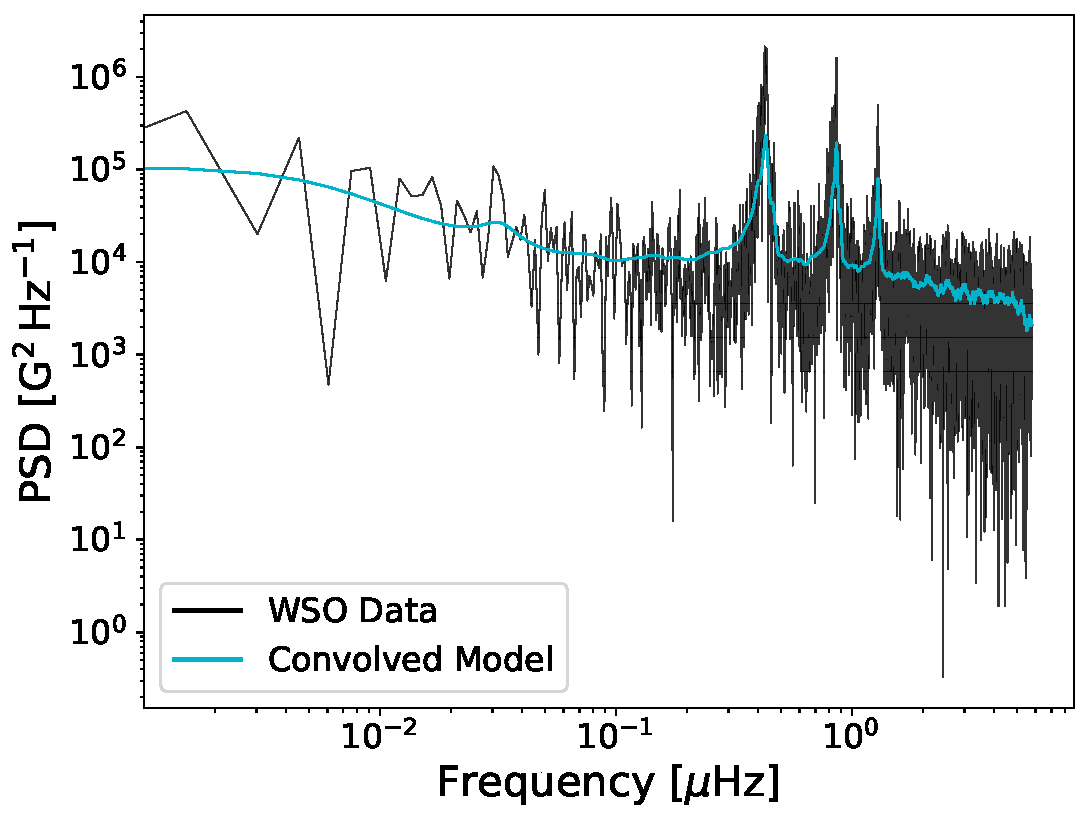
\includegraphics[width=\columnwidth]{WSO_PSD_model.pdf}
%	\caption{Full, modelled power spectrum of the WSO SMMF on logarithmic axes. The data are displayed in black and the convolved model using asymmetric Lorentzian peaks is shown in blue.}
%	\label{fig:WSO_PSD_fit}
%\end{figure}

\begin{figure}[ht!]
	\centering
	\subfloat[WSO \label{fig:WSO_PSD_fit}]
	{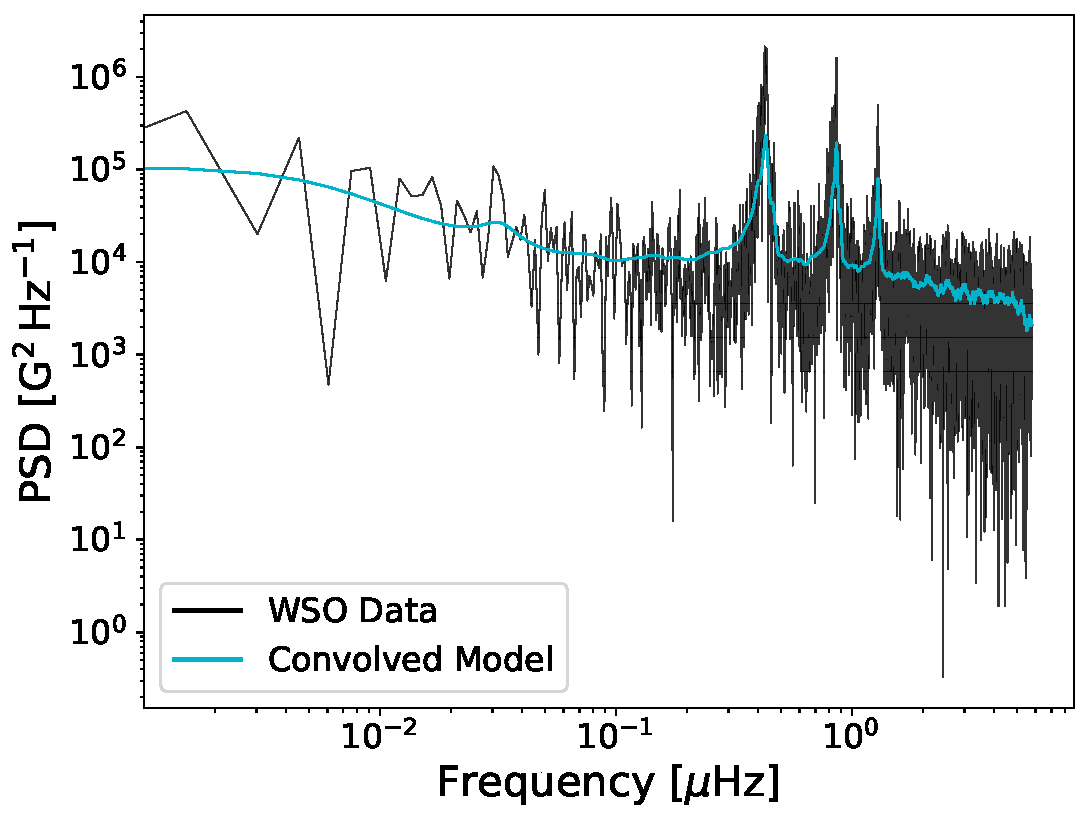
\includegraphics[width=0.47\columnwidth]{WSO_PSD_model.pdf}} 
	\qquad
	\subfloat[24-hr BiSON \label{fig:24h_BiSON_PSD_fit}]{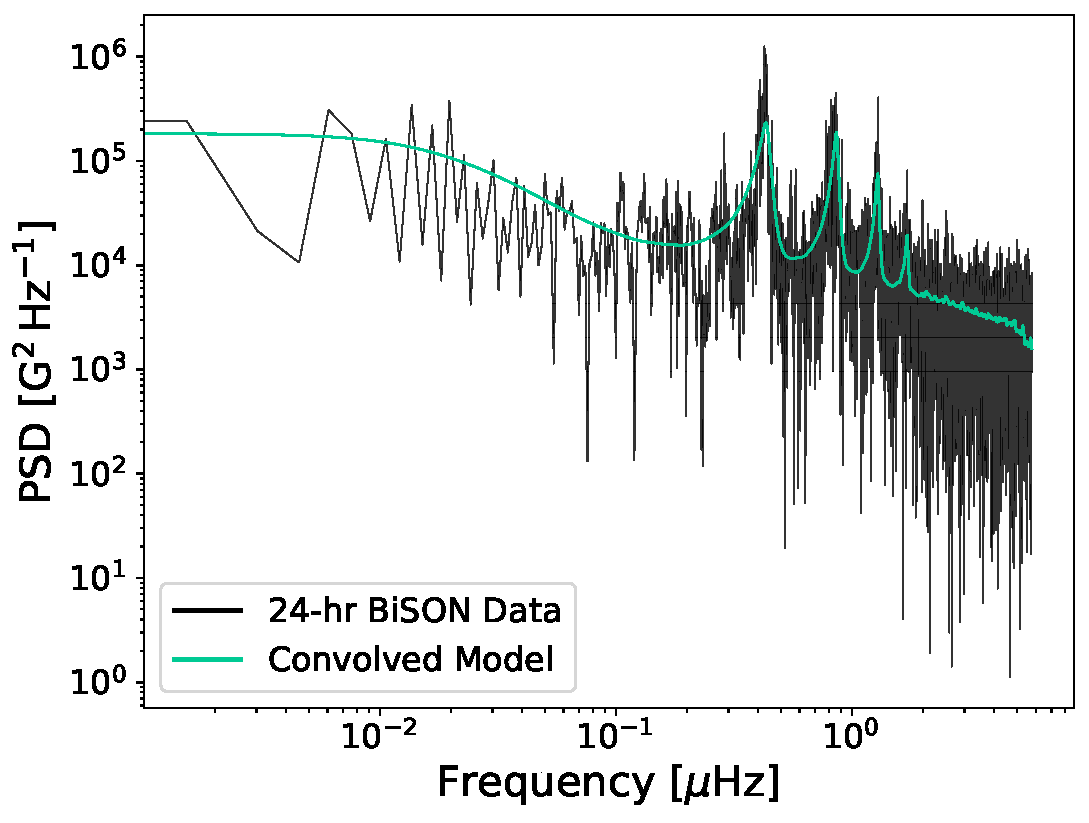
\includegraphics[width=0.47\columnwidth]{BiSON_24h_PSD_model.pdf}}
	\caption{Modelled power spectrum of (a) the WSO SMMF; (b) the daily-averaged BiSON SMMF, on logarithmic axes. The data are displayed in black and the convolved model using symmetric Lorentzian peaks is shown in blue and green, for WSO and BiSON, respectively.} 
	\label{fig:WSO_and_24h_BiSON_PSD_fit}
\end{figure}

The results of the fit to the daily-averaged \gls{bison} data are similar to those for the 40-second data, however there are a few differences which arise due to the different window functions and the realisations of the noise. We do however, generally, see a good agreement between the parameters. We see in Figure~\ref{fig:BiSON_PSD_40_vs_24} that there are differences between the daily-averaged and 40-second spectra; at low frequencies it is possible to see the differences in the realisations of the noise, and at higher frequencies we can see differences due to the window function aliasing. This plot shows the possible reasons why the parameters in Table~\ref{tab:WSO_SMMF_fit_params} may slightly differ from the results presented in Table~\ref{tab:PSD_fit_params}.

\begin{figure}[ht!]
	\centering
	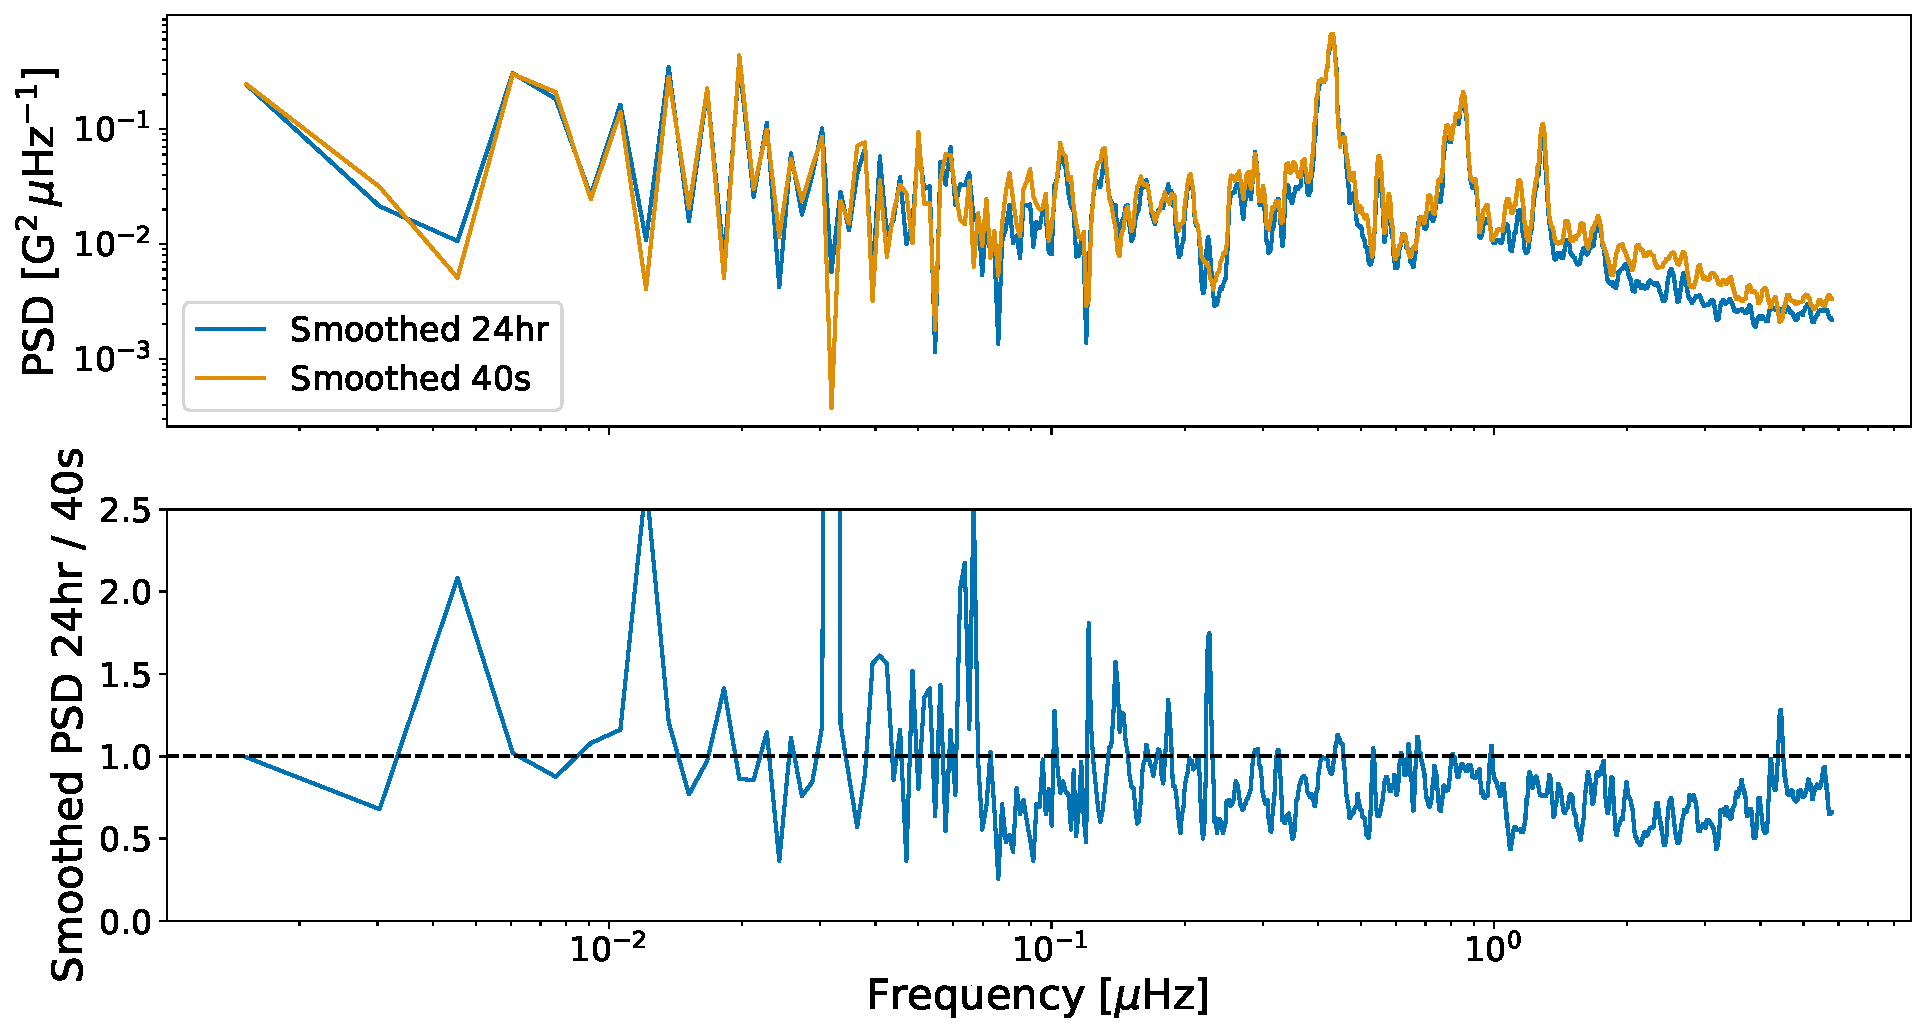
\includegraphics[width=\columnwidth]{BiSON_24h_vs_40s.pdf}
	\caption{A comparison between the power spectra produced using the daily-averaged BiSON data and the 40-second cadence BiSON observations. The top plot shows the log-smoothed power spectra of the daily-averaged data (blue) and the 40-second data (orange). The bottom panel show the ratio of the daily-averaged data power spectrum to the 40-second data power spectrum. The horizontal, dashed line indicates a ratio of 1.}
	\label{fig:BiSON_PSD_40_vs_24}
\end{figure}


The fit to the \gls{wso} power spectrum using a model with asymmetric Lorentzian profiles converged on an asymmetry parameter, but as with the 40-second analysis of the \gls{bison} data, we calculated the \gls{bic} values for both the symmetric and asymmetric model to determine which model to select. The \gls{bic} values for the \gls{wso} models using symmetric and asymmetric Lorentzian profiles were $\sim$47 and $\sim$55, respectively, and the \gls{bic} values for the \gls{bison} models using symmetric and asymmetric Lorentzian profiles were $\sim$55 and $\sim$63, respectively. In both cases, this highlighted that the models using the symmetric Lorentzian profiles were favoured, due to the lower \gls{bic} values. 

The rotation period in the \gls{wso} data is in agreement with that measured using \gls{bison} data to within 3$\sigma$, and this period implies a cycle-averaged latitude of around $\sim12^{\circ}$. This agrees with the conclusions drawn from our inferences of the \gls{bison} data, that the \gls{rm} source is linked to \glspl{ar}.


The linewidth from the \gls{wso} data implies a \gls{rm} lifetime of $175 \pm 13$~days, which is in the region of $\sim$25~weeks, or half a year. The \gls{wso} lifetime is in agreement with the 40-second \gls{bison} data. However, this lifetime is inconsistent with that measured using the daily-averaged \gls{bison} data. The lifetime measured using the daily-averaged \gls{bison} data is around 50\% smaller than that measured with the \gls{wso} data. A possible reason for this could be the differences arising from systematics in the fitting. When using the daily-averaged \gls{bison} data it is harder to accurately model the background because of the lower Nyquist frequency, hence we may be vulnerable to systematics impacting on the inferred widths as a higher fitted background would tend to produce narrower peak widths. %resolution differences of the two instruments, or more likely it is a by-product of the different regions within the photosphere that each instrument probes. 
These limits are still consistent however with the lifetime of large, strong \glspl{ar} \citep{schrijver_photospheric_1994, van_driel-gesztelyi_evolution_2015}. 

As with the \gls{bison} observations, the investigation of the \gls{wso} \gls{smmf} also indicates the origin of the \gls{smmf} is linked to \glspl{ar} and \glspl{mfc} that are long-lived on the solar disc and exist in active latitudes.



%%%%%%%%%%%%%%%%%%%%%%%%%%%%%%%%%%%%%%%%%%%%%%%%%%%%%%%%%%%%%%%%%%%%%
%%%%%%%%%%%%%%%%%%%%%%%%%%%%%%%%%%%%%%%%%%%%%%%%%%%%%%%%%%%%%%%%%%%%%
\section{Discussion}\label{sec:SMMF_artificial}



\subsection{Testing the Effects of Differential Rotation and Active Region Migration}
\label{sec:smearing}

We know the rotation period of \glspl{ar} varies throughout the solar cycle as a result of solar differential rotation and latitudinal migration. As we have inferred that the \gls{rm} component of the \gls{smmf} is likely linked to \glspl{ar} and \glspl{mfc}, we may therefore assume that the \gls{rm} component is also sensitive to these effects. Here we analyse the effect of migration and differential rotation on our ability to make inferences on the lifetime of the \gls{rm} component.

Several studies have modelled the solar differential rotation, and its variation with latitude and radius of the Sun \citep[see][for an in depth review of the literature on solar differential rotation]{beck_comparison_2000, howe_solar_2009}. Magnetic features have been shown to be sensitive to rotation deeper than the photosphere; therefore, in general, magnetic features can be seen to rotate with a shorter period than the surface plasma \citep{howe_solar_2009}.

\citet{chaplin_distortion_2008} analysed the effects of differential rotation on the shape of asteroseismic low-$l$ $p$ modes of oscillation, and showed that the consequence of differential rotation is to broaden the observed linewidth of a mode peak. The authors provide a model of the resultant profile of a $p$ mode whose frequency is shifted in time to be a time-average of several instantaneous Lorentzian profiles with central frequency $\nu(t)$, given by:
%
\begin{equation}
\langle P(\nu) \rangle \, = \, \frac{1}{T} \int^T_0 H \left( 1 \, + \, \left( \frac{\nu - \nu(t)}{\Gamma /2} \right)^2 \right)^{-1} dt \, .
\label{eq:stacked_lorentzians}
\end{equation}

The angled brackets indicate an average over time. $H$ and $\Gamma$ are the mode height (maximum power spectral density) and linewidth, respectively. The full period of observation is given by $T$.

\citet{chaplin_distortion_2008} also show that by assuming a simple, linear variation of the unperturbed frequency, $\nu_0$, from the start to the end of the time-series by a total frequency shift $\Delta\nu$ (see equation~(\ref{eq:linear_variation})),
%
\begin{equation}
\nu(t) \, = \, \nu_0 \, +  \Delta\nu \frac{t}{T} \, ,
\label{eq:linear_variation}
\end{equation}
%
the resultant profile of a $p$ mode can analytically be modelled by:
%
\begin{equation}
\langle P(\nu) \rangle \, = \, \frac{H}{2\epsilon} \arctan \left( \frac{2 \epsilon}{1 - \epsilon^2 + X^2 } \right) \, ,
\label{eq:atan_lorentzians}
\end{equation}
%
where $\epsilon$ and $X$ are defined in equation~(\ref{eq:epsilon}) and equation~(\ref{eq:X}):
%
\begin{equation}
\epsilon \, = \, \frac{\Delta\nu}{\Gamma} \, ;
\label{eq:epsilon}
\end{equation}
%
\begin{equation}
X \, = \, \frac{\nu - [\nu_0 + (\Delta\nu/2)]}{\Gamma /2} \, .
\label{eq:X}
\end{equation}

As the mode linewidths are broadened by this effect, we evaluated whether our ability to resolve the true linewidth of the \gls{rm} component, and hence its lifetime, was affected. To evaluate this we computed the broadened profiles given by both equation~(\ref{eq:stacked_lorentzians}) and equation~(\ref{eq:atan_lorentzians}), and fit the model for a single Lorentzian peak, to determine whether the linewidth is recovered.

In the first instance, we computed the broadened peak using equation~(\ref{eq:stacked_lorentzians}). Over the duration of the observations, we computed the daily instantaneous profile, $P(\nu(t))$. The time-averaged profile, $ \langle P(\nu) \rangle$, is a weighted average of each instantaneous profile, where the weights are given by the squared, daily-averaged \gls{smmf}, in order to allow a larger broadening contribution at times when the \gls{smmf} amplitude is large.

In the second instance, we computed the broadened peak using equation~(\ref{eq:atan_lorentzians}). Over the duration of the observations the daily frequency shift is computed, $\Delta\nu$. The time-averaged shift, $\Delta\nu$, is a weighted average, where again the weightings are given by the squared, daily-averaged \gls{smmf}.

To determine the shift in the rotation rate with migration, we used the model of the solar differential rotation as traced by magnetic features ($\Omega_m$) given by equation~(\ref{eq:diff_rot_freq}), where $\mu\,=\,\cos\theta$ and $\theta$ is the co-latitude \citep{snodgrass_magnetic_1983, brown_inferring_1989}:
%
\begin{equation}
\frac{\Omega_m}{2 \pi} \, = \, 462 - 74 \mu^2 - 53 \mu^4 \, \mathrm{nHz} \, .
\label{eq:diff_rot_freq}
\end{equation}

Finally, the time-dependence on the latitude of the active regions used the best-fitting quadratic model by \cite{li_latitude_2001}.

In both instances, the broadened peak was modelled as a single Lorentzian peak using equation~(\ref{eq:symm_lorentzian}), with a width equivalent to that which was inferred from modelling the \gls{bison} power spectrum. We used {\verb emcee } \citep{foreman-mackey_emcee_2013} to explore the posterior parameter space with priors similar to the fit to the full power spectrum.

Over the entire duration of the \gls{smmf} observations, the time-averaged profile was calculated, using equation~(\ref{eq:stacked_lorentzians}), and this is shown in Figure~\ref{fig:weighted_shift}. The broadened mode used the input parameters for the model using symmetric Lorentzians, outlined in Table~\ref{tab:PSD_fit_params}, however, with the background parameter set to zero. %For the input, we show the posterior width that resulted from the model to the \gls{bison}, which is shrunk due to the convolution process, rather than the more realistic width of $\sim 15\%$

By eye, the broadened profile does not appear to have a significantly larger linewidth. The input linewidth was $0.0264\pm0.0035~\upmu\mathrm{Hz}$, and the fit to the time-averaged broadened peak produced a linewidth of $0.0262^{+0.0038}_{-0.0037}~\upmu\mathrm{Hz}$. The linewidth of the broadened peak under this method was rather unchanged from that of the true peak, and both linewidths are within uncertainties of each other.

\vspace{1em}

\begin{table}[!ht]
	\begin{center}
		\caption{Input linewidth and the median posterior values of the Lorentzian model each simulation. Numbers in brackets denote uncertainties on the last 2 digits, and all uncertainties correspond to the 68\% credible intervals either side of the median.}
		\label{tab:shift_params}
		\begin{tabular}{l c c r}
			\hline
			%{} & 
			{\bf Input Value} & {\bf Weighted Fit} & {\bf Analytic Fit} & {\bf Unit} \\
			\hline
			
			
			%{} & 
			{0.0264$\pm0.0035$} & {$0.0262^{+0.0038}_{-0.0037}$} & {$0.0263^{+0.0038}_{-0.0037}$} & {$\upmu\mathrm{Hz} $} \\
			
			
			\hline
		\end{tabular}
	\end{center}
\end{table}


\begin{figure}[ht!]
	\centering
	\subfloat[Weighted \label{fig:weighted_shift}]
	{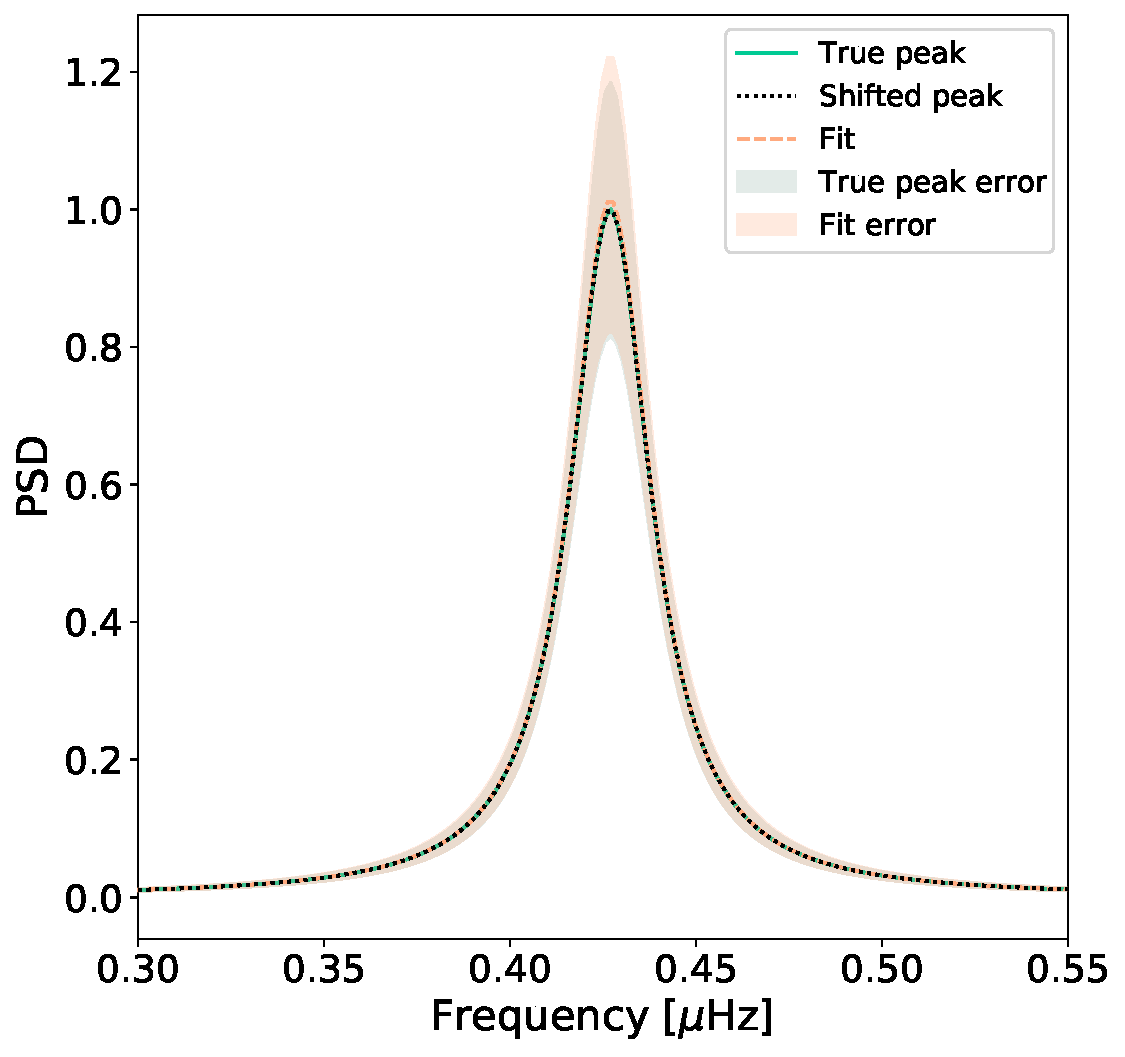
\includegraphics[width=0.47\columnwidth]{weighted_shifted_peak.pdf}} 
	\qquad
	\subfloat[Analytic \label{fig:atan_shift}]{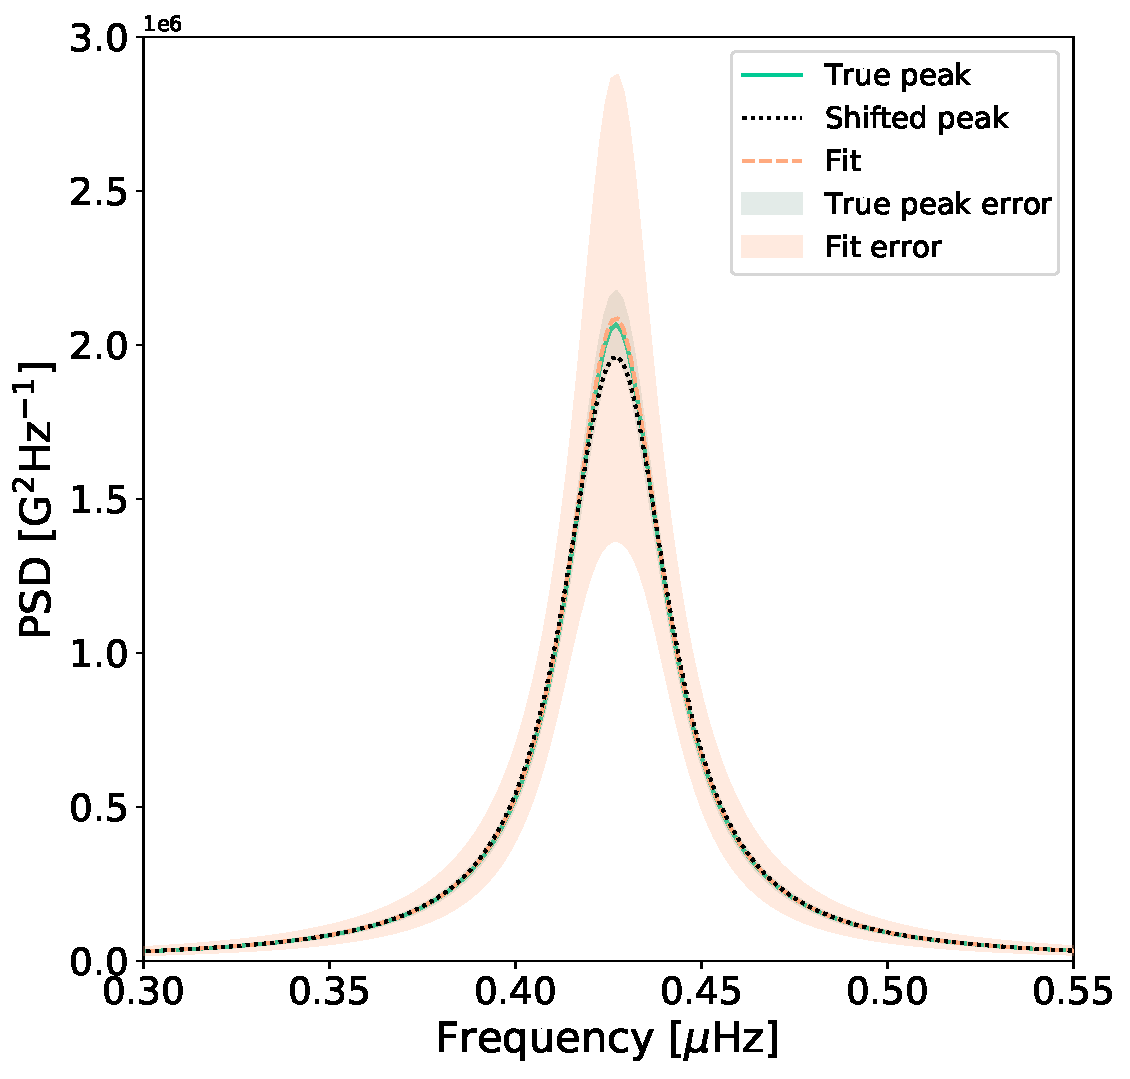
\includegraphics[width=0.47\columnwidth]{chaplin_shifted_peak.pdf}}
	\caption{(a) Shows the Lorentzian distribution peak before and after the time-averaged broadening, and the fit to the broadened peak. (b) Shows the peak distribution before and after the analytical broadening, and the fit to the broadened peak. In both plots the broadened peaks have been shifted by the relevant frequency to overlay them on top of the true $\nu_0$ for comparison.} \label{fig:shifted_peaks}
\end{figure}


The time-averaged frequency shift due to differential rotation was calculated, much in the same way as equation~(\ref{eq:stacked_lorentzians}), to be $\Delta\nu \, = \,0.01285 \, \upmu\mathrm{Hz}$. This shift was used to generate the broadened profile using equation~(\ref{eq:atan_lorentzians}). The broadened mode distribution also used the input parameters outlined in Table~\ref{tab:PSD_fit_params}, however, with the background parameter set to zero.

Similar to the numerically broadened peak, by eye, the analytically broadened profile does not appear to have a significantly larger linewidth (see Fig.~\ref{fig:atan_shift}). The input linewidth was $0.0264 \pm 0.0035 \, \upmu\mathrm{Hz} $, and the linewidth of the analytically broadened peak from the fit was $0.0263^{+0.0038}_{-0.0037} \, \upmu\mathrm{Hz} $, which was within the uncertainties of the linewidth of the input peak.

These results show that both numerically and analytically, the mode broadening effect of differential rotation and latitudinal migration does not affect our ability to resolve the linewidth of the peaks. Both broadening methods applied have been shown to have a negligible effect on the measured linewidth. This result provides confidence that the linewidth in Table~\ref{tab:PSD_fit_params} is the true linewidth of the \gls{rm} peaks, thus providing the correct lifetime for \gls{rm} component, unaffected by migration and differential rotation.





\subsection{Further Morphology of the SMMF using SDO/HMI Data}
\label{sec:SMMF_morphology}


In Chapter~\ref{chap:rmode} we acquired \gls{sdo/hmi} full-disc magnetograms, using the {\verb SunPy } python module \citep{barnes_sunpy_2020}, to support our investigations into Rossby waves (see next chapter for details).

%Here we use \gls{sdo/hmi} data to show how the SMMF is broken down into its hemispheric behaviour and how that affects the full-disc SMMF...
%
%
%
%\begin{figure}[!ht]
%	\centering
%	\subfloat[...]{
%		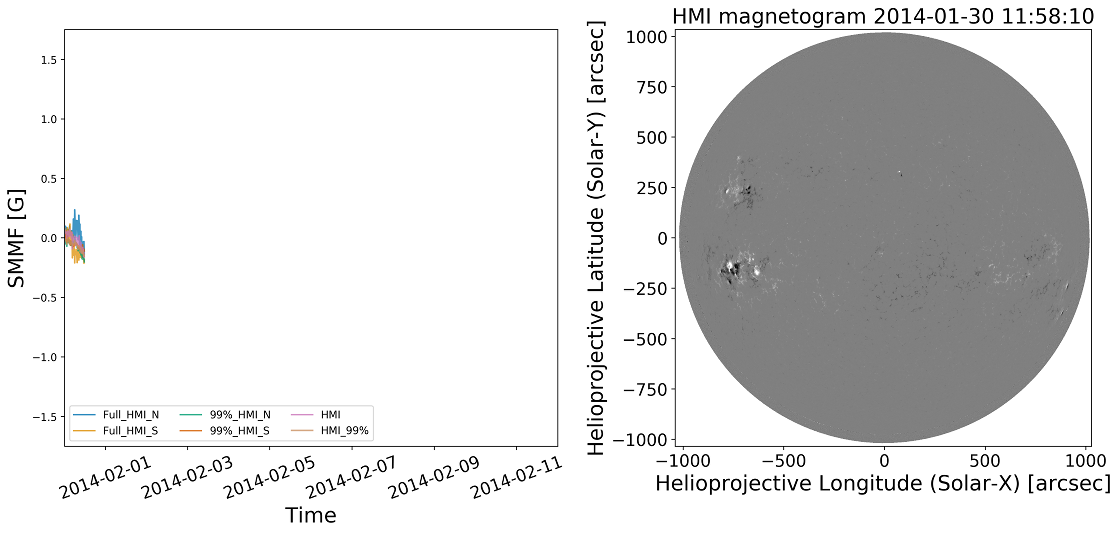
\includegraphics[width=0.9\columnwidth]{HMI_20140130_120000_rescaled.png}
%		\label{fig:20140130}}
%	
%	\qquad
%	
%	\subfloat[...]{
%		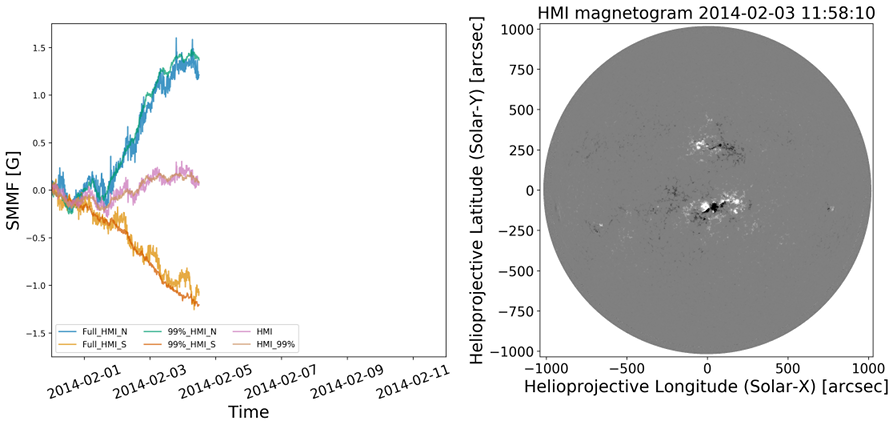
\includegraphics[width=0.9\columnwidth]{HMI_20140203_120000_rescaled.png}
%		\label{fig:20140203}} \\
%	
%	\qquad
%	
%	\subfloat[...]{
%		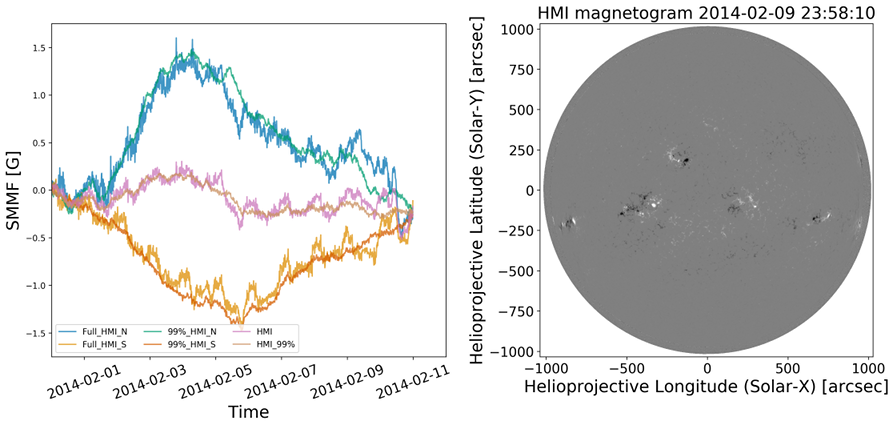
\includegraphics[width=0.9\columnwidth]{HMI_20140210_000000_rescaled.png}
%		\label{fig:20140210}}
%
%	
%	\caption{...}
%	\label{fig:HMI_frames_2014}
%\end{figure}
%
%
%
%\begin{figure}[!ht]
%	\centering
%	\subfloat[...]{
%		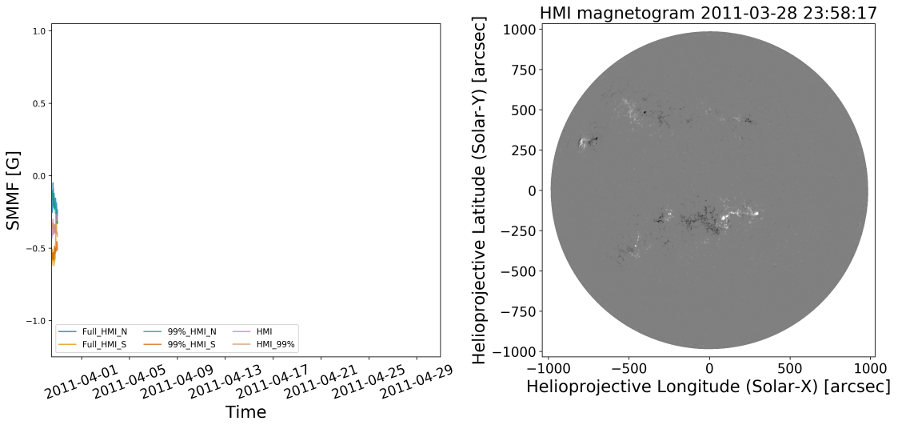
\includegraphics[width=0.9\columnwidth]{HMI_20110329_000000_rescaled.png}
%		\label{fig:20110329}}
%	
%	\qquad
%	
%	\subfloat[...]{
%		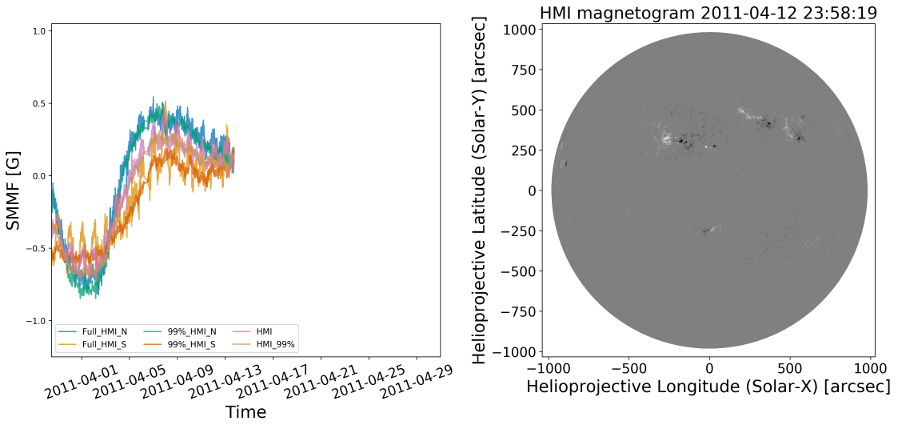
\includegraphics[width=0.9\columnwidth]{HMI_20110413_000000_rescaled.png}
%		\label{fig:20110413}} \\
%	
%	\qquad
%	
%	\subfloat[...]{
%		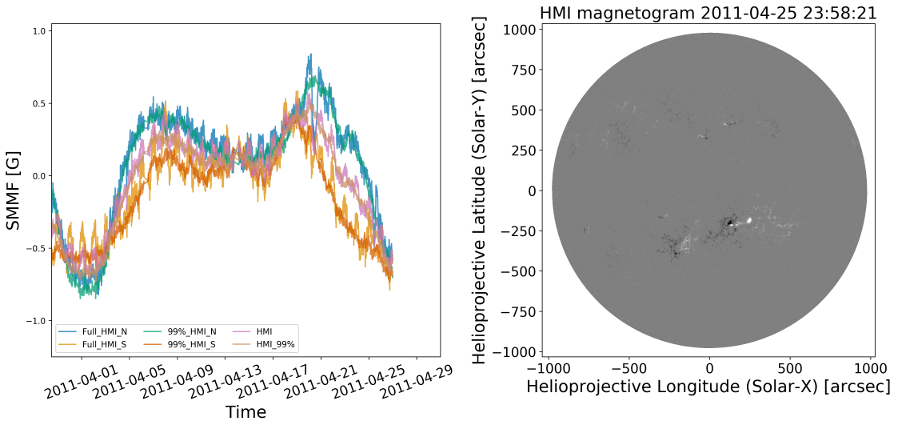
\includegraphics[width=0.9\columnwidth]{HMI_20110426_000000_rescaled.png}
%		\label{fig:20110426}}
%	
%	
%	\caption{...}
%	\label{fig:HMI_frames_2011}
%\end{figure}
%
%
%We see here a number of key observations:
%
%During periods of high activity, when both the Northern and Southern hemispheres have strong \gls{ar}s in phase with each other, they provide strong contributions to the hemispheric MF, which nearly cancel out in the total SMMF.
%
%During periods where \gls{ar}s appear on the disc that are not in phase with each other, then they provide strong contributions to the hemispheric MF and total SMMF.
%
%Most surprisingly is that we do see that the SMMF is large when regions of obvious sunspots, plages, and network are not on the disc, or are waxing or waning on the disc, providing support for the flux distributed around the \gls{ar}s ()i.e. those trailing the \gls{ar}s) to 


Owing to having the \gls{sdo/hmi} magnetograms, which provided the capability to separately analyse the Northern and Southern Hemispheres' \gls{mmf} contribution to the \gls{smmf} during the rising phase of Cycle 24 in 2011 and during solar maximum in 2014, we also investigated whether there were hemispheric differences in the data, which resulted from the opposite polarities at high latitudes and towards the poles. This served as a further analysis into other timescales which may exist in the \gls{smmf}. In particular, we investigated whether the \gls{smmf} exhibited an anti-correlation between the two hemispheres due to the oppositely polarised field near the polar regions, as found in synoptic charts, on a time-scale of the solar cycle.

To support this investigation, we acquired the synoptic charts from \gls{sdo/hmi}. It was possible to average the signal over the Northern and Southern Hemispheres of the synoptic charts, as well as the full solar surface, thus providing a comparison to the hemispheric \gls{mmf} and the full disc \gls{smmf}.

To compare the magnetogram data to the synoptic charts, we smoothed the separately averaged Northern and Southern Hemispheres' \gls{mmf} and the full-disc \gls{smmf} signals using a box-car filter with a window width of a Carrington period, i.e. $\sim 27$~days. The resultant time series was plotted along with the hemispheric mean of the synoptic charts from \gls{sdo/hmi}. Figure~\ref{fig:HMI_MF_vs_synoptics} shows the resultant smoothed hemispheric \gls{mmf} and full-disc \gls{smmf} along with the average of the synoptic charts.

\begin{figure}[!ht]
	\centering
	\subfloat[2011 \label{fig:HMI_2011_MF}]{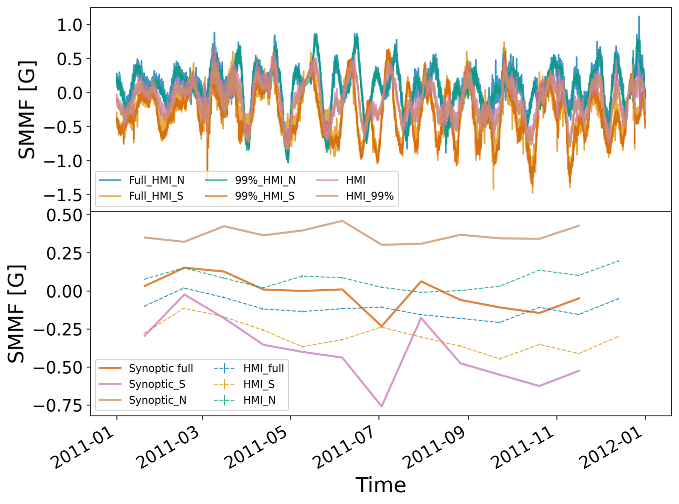
\includegraphics[width=0.75\columnwidth]{HMI_MF_vs_synoptic_2011_rescaled.png}} 
	\qquad
	\subfloat[2014 \label{fig:HMI_2014_MF}]{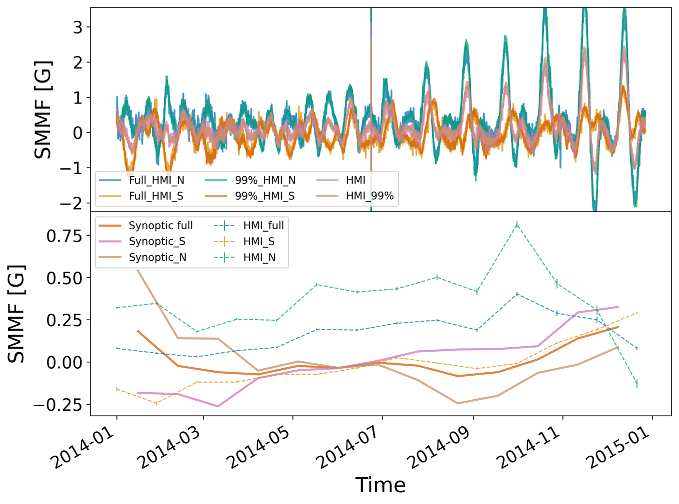
\includegraphics[width=0.75\columnwidth]{HMI_MF_vs_synoptic_2014_rescaled.png}}
	\caption{Investigations of timescales in the SDO/HMI magnetograms over 2011 and 2014. Both plots show in the top panel, the hemispheric \gls{mmf} and full-disc \gls{smmf} from the magnetograms. The lower panel of each plot displays a comparison between the hemispheric and full-disc mean of the synoptic charts, compared to the box-car smoothed \gls{mmf} from the magnetograms. N: Northern hemisphere; S: Southern hemisphere. Full HMI: considers the full solar disc; 99 HMI: considers only the inner 99\% of the solar disc, by radius.}
	\label{fig:HMI_MF_vs_synoptics}
\end{figure}

We can see from Figure~\ref{fig:HMI_MF_vs_synoptics} that there does exist a longer timescale in the hemispheric \gls{mmf} when we average out the effects of the \gls{rm} component. This is visible from the reversal of the field polarity in 2014. This longer timescale component resembles the average of the synoptic charts, and shows the secular variation which is contributed by the solar dipole at high latitudes. This timescale is the solar activity period and can be seen particularly in Figure~\ref{fig:HMI_2014_MF}. We see the beginning of a the magnetic field reversal at around solar maximum, in mid-2014, with the onset of the ``rush to the poles" after solar maximum \citep{wilson_solar_1994, mcintosh_what_2019}.

Interestingly, the field reversal was located during different epochs when comparing the synoptic chart data to the visible disc, hemispheric \gls{mmf} data, and was delayed in the hemispheric \gls{mmf} by around 7 Carrington rotations. Naturally, when the full-disc averaged \gls{smmf} was smoothed, the \gls{rm} component was averaged out, resulting in a near-flat line. This was however expected as it was the average of the opposite hemispheres, and is consistent with the synoptic charts.


%%%%%%%%%%%%%%%%%%%%%%%%%%%%%%%%%%%%%%%%%%%%%%%%%%%%%%%%%%%%%%%%%%%%%
%%%%%%%%%%%%%%%%%%%%%%%%%%%%%%%%%%%%%%%%%%%%%%%%%%%%%%%%%%%%%%%%%%%%%
\section{Conclusion}\label{sec:SMMF_conclusion}

We have presented, for the first time, a frequency-domain analysis of over 20~years of high-cadence (40-second) \gls{bison} observations of the \gls{smmf}.

Observations of the \gls{smmf} were computed from the Zeeman split D1 line of Potassium at $\sim$770~nm, as measured by the Sutherland node of \gls{bison}. The observations covered 7643~days over the period from 1992--2012 with a cadence of 40~seconds. A frequency-domain analysis of the \gls{smmf} was performed; the short cadence and long baseline of observations gave a fine frequency resolution in the power spectrum up to a high Nyquist frequency, allowing us to probe the elements that underpin the observed \gls{smmf}.

The duty cycle for the 40-second cadence observations was very low, hence the effect of the low fill on the power spectrum of the \gls{smmf} was investigated to help inform how to best model the full power spectrum. We highlighted that although there appeared to exist a red-noise-like, stochastic background component in the power spectrum, this was a feature originating from power aliasing due to the low duty cycle of the observations.

In the power spectrum, there was a strong peak at a frequency corresponding to the solar rotation, denoted the \gls{rm} signal/component. It was also demonstrated that the low duty cycle aliased the power of the prominent peak due to the solar rotation to higher frequencies, which provided several copies of this peak at higher frequencies.

Using a model comprising of a series of Lorentzian peaks to model the \gls{rm} signal, a Harvey function to account for lower frequency drifts, and shot-noise limit, which was convolved with the Fourier transform of the window function to account for the low duty cycle artefacts, we modelled the full power spectrum and measured the properties of the \gls{rm} signal.

It was demonstrated that the convolution process affected the total power in the model, thus careful treatment was taken to ensure Parseval's theorem was obeyed. In addition, it was shown that the width of the posterior distributions for the parameters had been systematically underestimated, as a result of the convolution process, because we do not account explicitly for the impact of the window function convolution on the covariance of the data. We could not resolve this, but simulated data provided a comparison between a model with and without convolution which was used to provide a correction to account for the systematic underestimate of the credible regions of the posterior when modelling the power spectrum of the observed \gls{bison} \gls{smmf}.

A comparative study was conducted on the \gls{wso} data over the same observational epoch and the modelled power spectrum provide results that were in agreement with those measured in the \gls{bison} power spectrum.

To further investigate the \gls{smmf} and our ability to infer the properties of the source, we used simulations to analyse the effects of differential rotation and \gls{ar} migrations on our ability to measure the linewidth.

Finally, a short investigation into the \gls{smmf} as measured by \gls{sdo/hmi} was conducted. Smoothing the data over the solar rotation period for both Northern and Southern hemispheres, separately, uncovered that the hemispheres display a longer variation, in accordance with the solar activity cycle, similar to that of the full-disc synoptic maps.

We leave the reader with the following points:

\begin{enumerate}
	\item{We have shown that there does not exist a short time-scale component in the \gls{smmf}, and the emergence of a red-noise-like signal in the power spectrum was due to the low duty cycle of the \gls{bison} observations.}
	
	\item{By modelling the peak of the \gls{rm} signal as a symmetric Lorentzian profile, we found that the peak has a central frequency of $0.4270\pm0.0018\,\upmu\mathrm{Hz}$. This measurement of the central frequency allowed us to infer the sidereal period of the \gls{rm} signal to be $25.23\pm0.11$~days. This rotation suggests a magnetic feature, cycle-averaged latitude of $\sim 12^{\circ}$, thus linking the source to active bands of latitude on the Sun.}
	
	\item{The lifetime of the source of the \gls{rm} component was inferred from the linewidth of the Lorentzian peaks to be $139.6\pm18.5$~days, which is in the region of $\sim20\pm3$~weeks.}
	
	\item{As a comparison, the power spectrum of the \gls{smmf} measured by \gls{wso} was also modelled and the linewidth and central frequency of the \gls{rm} component were measured. The results were generally consistent with those from the \gls{bison} data, and the conclusions inferred were in accordance.}
	
	\item{The measured properties of the \gls{rm} component of the \gls{smmf} are consistent with \glspl{ar}. The literature advises that sunspots are not the origin of the \gls{smmf}, here we suggest that \glspl{ar} and \glspl{mfc} are the source of the dominant, rotation signal in the \gls{smmf}, that are long-lived on the solar disc and exist in active latitudes.}
		
	\item{We have shown that our ability to determine the linewidth and hence lifetime of the \gls{rm} modes was unaffected by \gls{ar} migration and differential rotation.}
	
	%\item{Through simulating artificial \gls{smmf} data, we explored the source of the asymmetry in the model. We believe the asymmetry is a result of the phase interference between localised, near-surface regions of \glspl{mfc}.}
	
	\item{Finally, a short investigation into the hemispheric contributions to the \gls{smmf}, using data from \gls{sdo/hmi}, showed there is a longer-term variation which underpins the \gls{smmf}, in accordance with the activity cycle and polar field reversals.}
\end{enumerate}


At the time of writing, only two more of the \gls{bison} nodes were actively measuring the \gls{smmf} (Las Campanas and Narrabri), and their measurements of the \gls{smmf} are not as stable as those measured by the Sutherland node. Sutherland has not been measuring the \gls{smmf} since 2013, however. Plans are in place to re-acquire these data in Sutherland and elsewhere, such that the frequency resolution can be further increased with a longer baseline, allowing for more accurate inferences on the \gls{smmf} morphology.

With more time on the project, it would also be useful to develop a technique similar to \citet{kutsenko_contribution_2017} and \citet{bose_variability_2018}, which allows the \gls{smmf} to be dissected into regions and features on the disc.









%%%%%%%%%%%%%%%%%%%%%%%%%%%%%%%%%%%%%%%%%%%%%%%%%%%%%%%%%%%%%%%%%%%%%%%%%%%%%
%%%%%%%%%%%%%%%%%%%%%%%%%%%%%%%%%%%%%%%%%%%%%%%%%%%%%%%%%%%%%%%%%%%%%%%%%%%%%
%%%%%%%%%%%%%%%%%%%%%%%%%%%%%%%%%%%%%%%%%%%%%%%%%%%%%%%%%%%%%%%%%%%%%%%%%%%%%
%OLD REMOVED BIT ON THE ASYMMETRY INVESTIGATION...
%%%%%%%%%%%%%%%%%%%%%%%%%%%%%%%%%%%%%%%%%%%%%%%%%%%%%%%%%%%%%%%%%%%%%%%%%%%%%
%%%%%%%%%%%%%%%%%%%%%%%%%%%%%%%%%%%%%%%%%%%%%%%%%%%%%%%%%%%%%%%%%%%%%%%%%%%%%
%%%%%%%%%%%%%%%%%%%%%%%%%%%%%%%%%%%%%%%%%%%%%%%%%%%%%%%%%%%%%%%%%%%%%%%%%%%%%
%\subsection{Asymmetry in the Power Spectrum}
%\label{sec:asymmetry}
%
%We have shown that the \gls{bison} and \gls{wso} \gls{smmf} power spectra are best modelled with asymmetric Lorentzian profiles. In this section, we investigate the cause of this asymmetry. 
%
%An initial hypothesis on the origin of the asymmetry was the migration of active regions towards the equator with the progression of the solar cycle. This is illustrated clearly by the asymmetry in the rotation frequencies of sources at latitudes sampled from a \gls{kde} of the SSN, in combination with models for the differential rotation \citep{snodgrass_magnetic_1983} and equatorial migration \citep{li_latitude_2001}, shown in Figure~\ref{fig:KDE_lats}. The migration of \glspl{ar} towards the equator produces a clear, negatively asymmetric distribution of rotation frequencies, which has a longer tail at lower frequencies, in accordance with the asymmetry of the Lorentzian peaks in the \gls{bison} and \gls{wso} power spectra. If the total power spectrum is the sum of the power spectra for each contributing source, which have central frequencies following the distribution shown in Figure~\ref{fig:KDE_lats}, then we may expect to see this same asymmetry manifested in the power spectrum.
%
%To investigate migration as a source of the asymmetry, we used artificial data which were created to simulate the differential rotation and migration of active regions during the solar cycle. This was done by using two simplistic models, independently and in combination, for the transit of \gls{ar} sources across the solar disc: (a) a single \gls{ar} - ``cosine model", or (b) two regions of opposite polarity, such as sunspot pairs or a \gls{bmr} - ``sign-change model". In each case, the source(s) ingress the visible disc from one limb, traverse across the disc, and egress the other limb. The methodology involved with generating the simulated data is discussed in greater detail in Appendix~\ref{app:SMMF_sims}, and here we discuss the outcomes.
%
%\begin{figure}[ht!]
%	\centering
%	\subfloat[KDE of SSN \label{fig:kde}]
%	{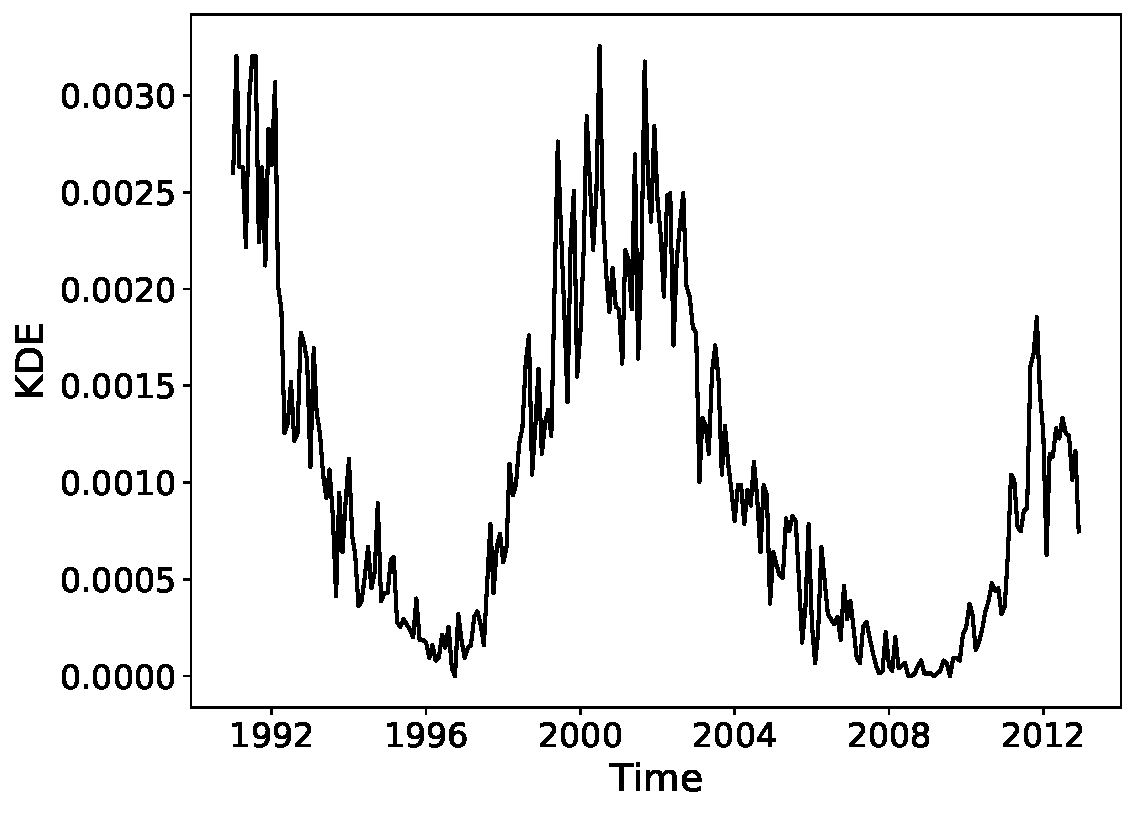
\includegraphics[width=0.47\columnwidth]{monthly_SSN_KDE.pdf}} 
%	\qquad
%	\subfloat[Histogram of source rotation frequency \label{fig:lats}]{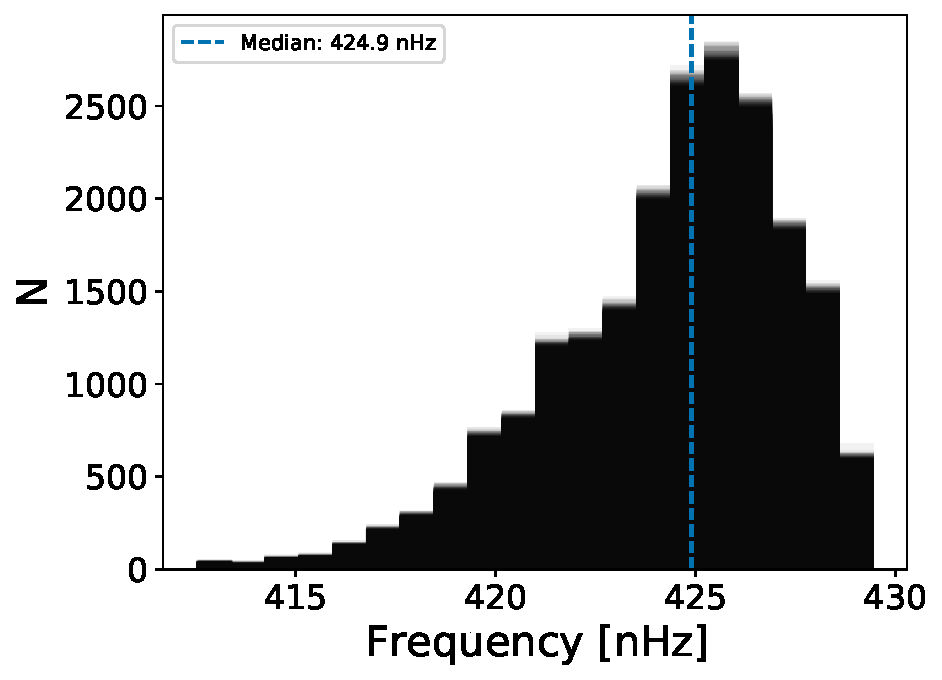
\includegraphics[width=0.47\columnwidth]{lat_hist.pdf}}
%	\caption{(a) Shows the KDE of the monthly averaged sunspot number used to draw samples of source seed times; (b) distribution of the rotation frequency of sources sampled from the KDE, after using the model for the migration and differential rotation.} 
%	\label{fig:KDE_lats}
%\end{figure}
%
%Three separate models for the migration of \glspl{ar} towards the equator were used in the simulations and they are shown in Figure~\ref{fig:artificial_sim_lats}. The quadratic model was taken from \citet{li_latitude_2001}, which represents a `typical' migration of \glspl{ar}, and the linear and exponential models were parametrised to provided opposite extremes for a slower and faster migration towards the equator, respectively. The aim of this was to investigate whether varying the migration rate affected the asymmetry. Each migration model is given in equation~(\ref{eq:quad_lats}), (\ref{eq:lin_lats}), and (\ref{eq:exp_lats}), where $t$ is the time since the start of the cycle, in years:
%
%\begin{equation}
%\lambda_{q} = 0.0893t^2 - 2.8t + 27.24 \, ;
%\label{eq:quad_lats}
%\end{equation}
%
%\begin{equation}
%\lambda_{l} = -1.84t + 27.24 \, ;
%\label{eq:lin_lats}
%\end{equation}
%
%\begin{equation}
%\lambda_{e} = 20.24 e^{-t/2} + 7 \, .
%\label{eq:exp_lats}
%\end{equation}
%
%In Figure~\ref{fig:artificial_sim_plots} we also note that for each model of the migration, we saw a different median rotation frequency in the distribution, which was lower for the slower migration, and higher for the faster migration. This was expected, due to the differential rotation, but it shows that the measured central rotation frequency of the \gls{smmf} power spectrum was sensitive to the migration and tells us something about the source. This also suggested that the \gls{rm} component on the \gls{smmf} power spectrum was consistent with a faster migration model.
%
%\begin{figure}[!ht]
%	\centering
%	\subfloat[Migration Models]{
%		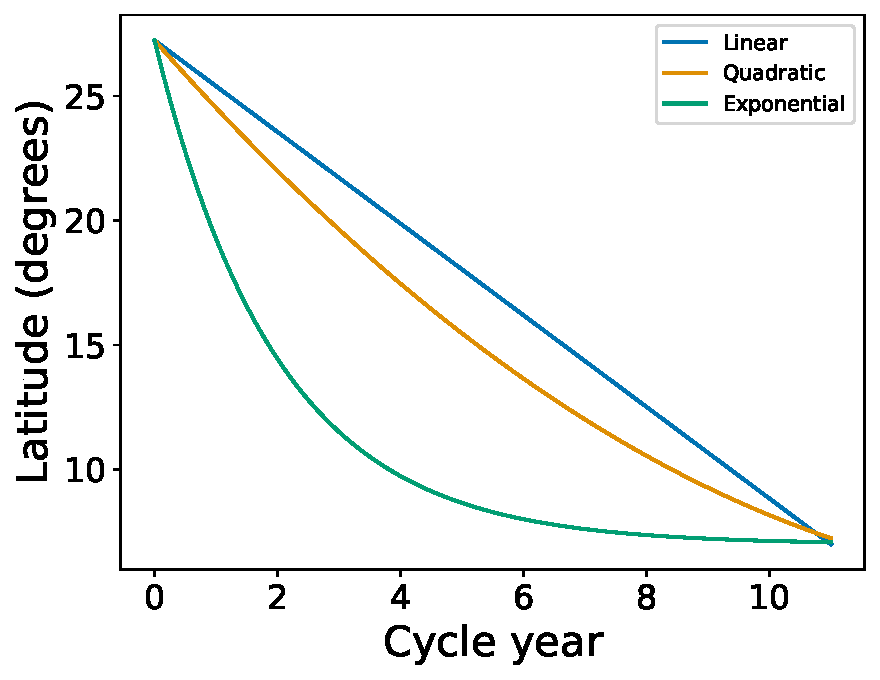
\includegraphics[width=0.45\columnwidth]{lats.pdf}
%		\label{fig:artificial_sim_lats}}
%	\qquad
%	\subfloat[Linear Migration]{
%		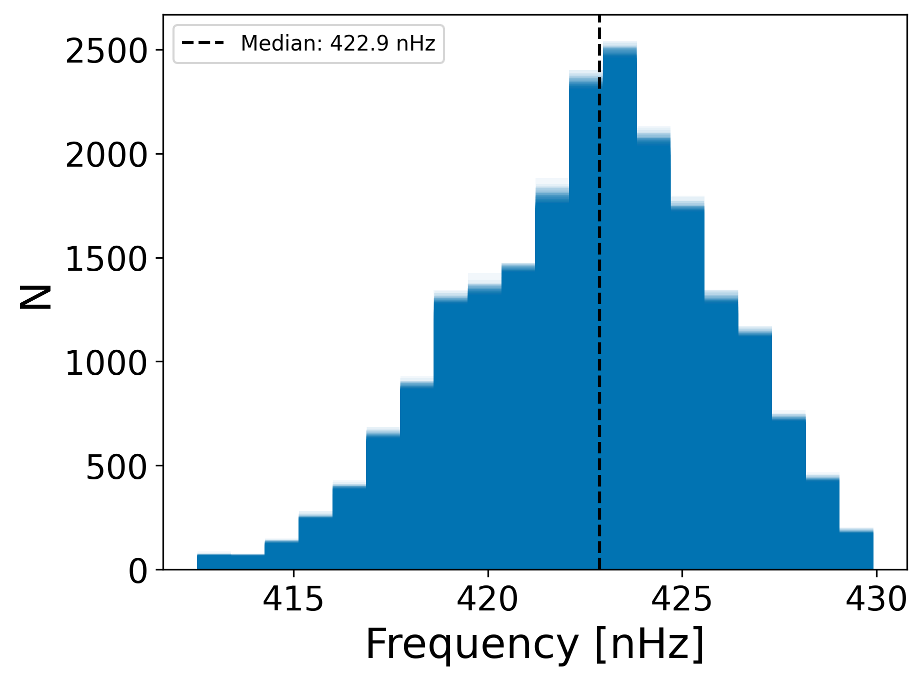
\includegraphics[width=0.45\columnwidth]{lin_rescaled.png}
%		\label{fig:artificial_sim_lin}} \\
%	
%	\qquad
%	
%	\subfloat[Quadratic Migration]{
%		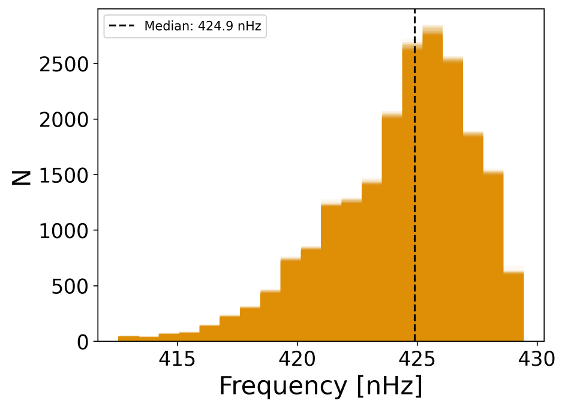
\includegraphics[width=0.45\columnwidth]{quad_rescaled.png}
%		\label{fig:artificial_sim_quad}}
%	\qquad
%	\subfloat[Exponential Migration]{
%		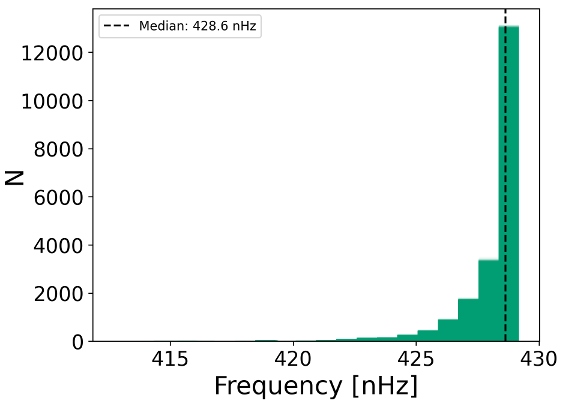
\includegraphics[width=0.45\columnwidth]{exp_rescaled.png}
%		\label{fig:artificial_sim_exp}}
%	
%	\caption{(a) Shows the latitudinal migration model as a function of time for each model; (b)-(d) shows the distribution of the rotation frequencies of sources sampled from the KDE for linear, quadratic, and exponential migration models, respectively.}
%	\label{fig:artificial_sim_plots}
%\end{figure}
%
%The simulations were run with 15 different configurations which used the three migration models combined with five models for the source transits across the visible disc. The five transit models were composed of the cosine model, sign change model, and combinations of the cosine and sign change models in ratios of 5:95, 10:90, and 20:80 (see Appendix~\ref{app:SMMF_sims} for further details). In each case, 250 simulations were performed in order to produce a limit spectrum by co-adding spectra from each independent realisation. Each limit spectrum was then modelled with a series of Lorentzian peaks sharing a global asymmetry parameter, and the resultant asymmetry values are shown in Figure~\ref{fig:artificial_asymm}.
%
%\begin{figure}[ht!]
%	\centering
%	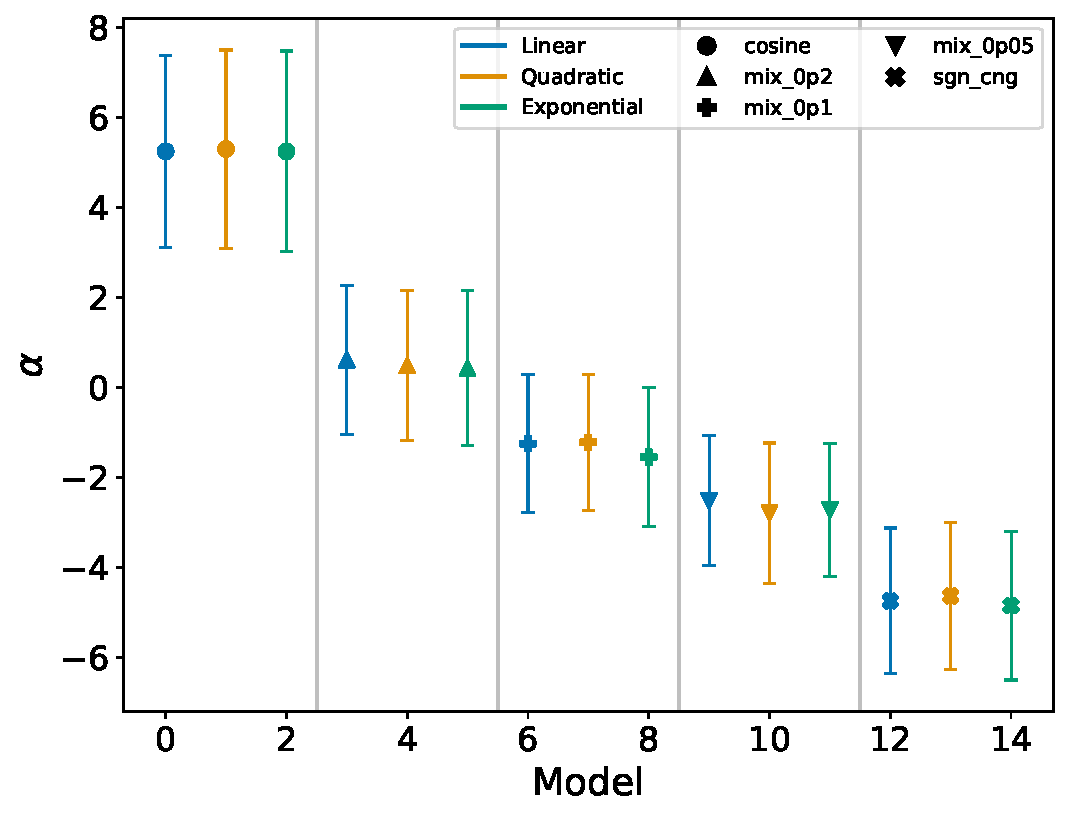
\includegraphics[width=0.85\columnwidth]{artificial_fit_asym.pdf}
%	\caption{The median value of the fitted global asymmetry parameter for several simulations of artificial data. The colour represents the migration model used: linear:blue; quadratic:orange; exponential: green. The marker represents the source model used: cosine:circle; sign change:cross; combinations of the cosine and sign change models in ratios of $5:95$:downwards triangle; $10:90$:plus; $20:80$:upwards triangle.}
%	\label{fig:artificial_asymm}
%\end{figure}
%
%It was immediately clear that the choice of migration model had no significant effect on the asymmetry of the Lorentzian peaks, hence we are able to rule out \gls{ar} migration as the origin of the asymmetry observed. It was therefore likely-incorrect to suggest that the total power spectrum was the sum of power spectra for each individual source, because this neglects the interference between sources in the time domain. However, Figure~\ref{fig:artificial_asymm} did show an obvious difference between the way the different models of the sources have asymmetry manifested in their spectra.
%
%This links to a still-open debate in helioseismology, on the source of asymmetry of the modes in the power spectra, and the asymmetry reversal between the observations in intensity and Doppler velocity. Asymmetry is regularly observed in $p$ modes of oscillation in helioseismic data and we observe a difference in the sign of the asymmetry term which is negative for Doppler velocity observations (i.e. more power in the low-frequency wing of the mode) and positive for measurements made in intensity (i.e. more power in the high-frequency wing of the mode) \citep{duvall_asymmetries_1993, chaplin_depth_1999, howe_validation_2015, basu_asteroseismic_2017}.
%
%There are believed to be two main causes of asymmetry in acoustic modes:
%
%\begin{enumerate}
%	\item{The spatially localised nature of the excitation source of acoustic modes in the near-surface layers of the outer convection zone and the interference between multiple waves that have accumulated a phase difference since their emission. This source of asymmetry is believed to dominate in Doppler velocity observations.}
%	
%	\item{The correlation between the convective granulation (i.e. correlated noise) and the signal from the modes themselves, or the correlation between the excitations of one mode to another. This source of asymmetry is believed to dominate in intensity observations due to the lower signal-to-noise ratio.}
%\end{enumerate}
%
%Here, however, we are not observing standing waves, but instead a rotationally modulation signal, therefore the explanation is slightly different. We suspected that the reason for the asymmetry could be due to interference between multiple sources, produced by a phase difference between source. To test this, we simulated differing numbers of sources to observe whether this resulted in a variation in the asymmetry. The results of this investigation are summarised in Figure~\ref{fig:asymm_sources}.
%
%\begin{figure}[ht!]
%	\centering
%	\subfloat[Limit spectra comparison for different numbers of simulated sources \label{fig:asymm_PSDs}]
%	{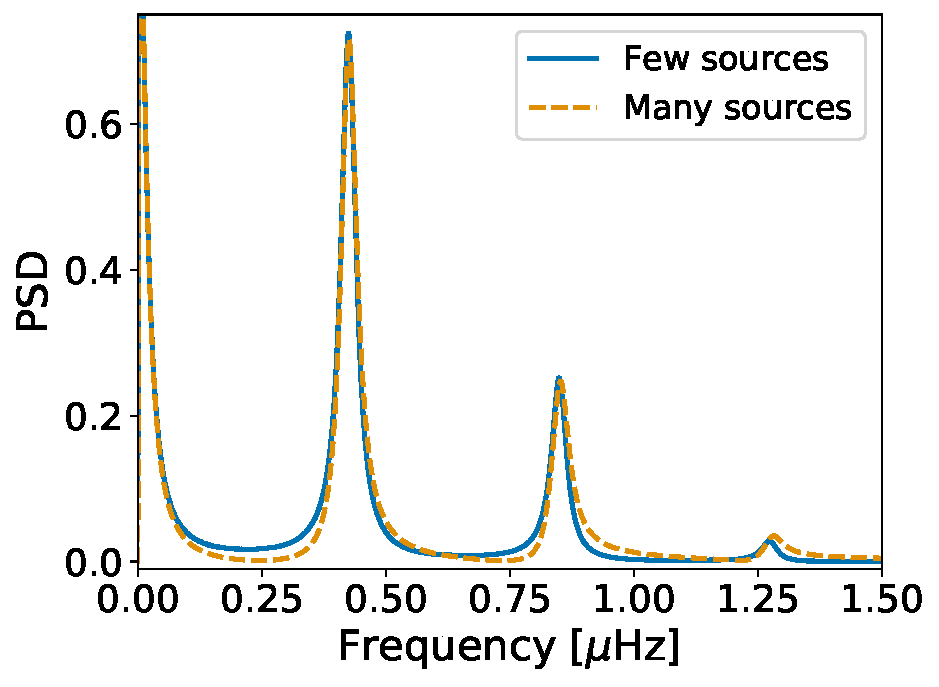
\includegraphics[width=0.48\columnwidth]{asymm_PSDs.pdf}} 
%	\qquad
%	\subfloat[Asymmetry parameter comparison for different numbers of simulated sources \label{fig:asymm_alphas}]{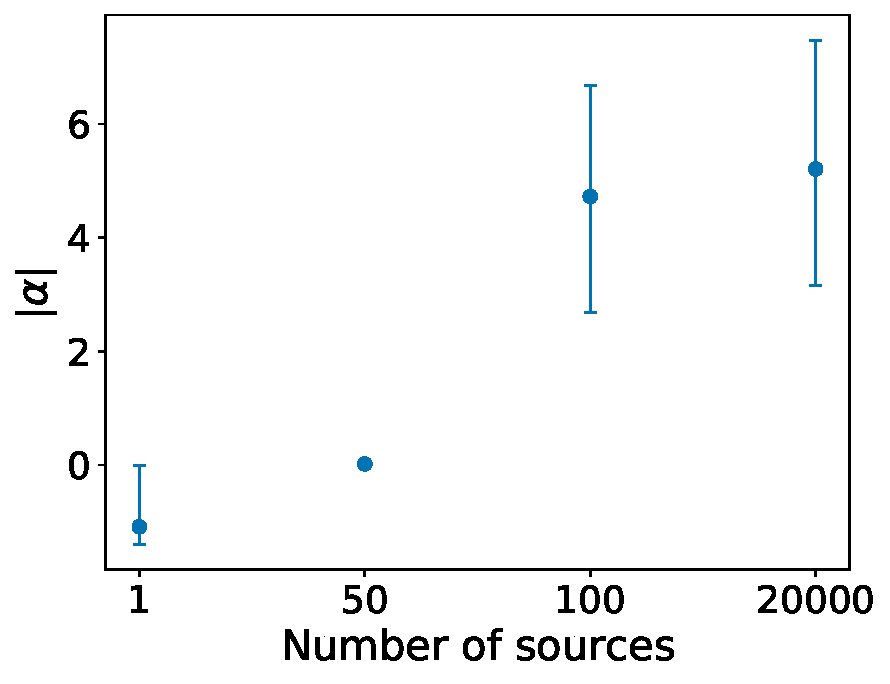
\includegraphics[width=0.46\columnwidth]{asymm_alphas.pdf}}
%	\caption{A comparison between the asymmetry in the power spectra for differing numbers of simulated sources. (a) Shows a direct comparison between the limit spectra for a single simulated source versus 100 simulated sources under the `cosine' model. (b) Shows a comparison of the median value fitted global asymmetry parameter for several numbers of simulated sources.} 
%	\label{fig:asymm_sources}
%\end{figure}
%
%Figure~\ref{fig:asymm_sources} shows that the asymmetry induced in the power spectrum has a clear relationship with the number of simulated sources. In Figure~\ref{fig:asymm_alphas}, it appears that this relationship follows a sigmoid shape, whereby the asymmetry increases up to a limiting value, and further sources will no longer have a significant effect on the asymmetry observed. We understand that in these simulations, whereby sources are simulated over $\sim 7000$~days with e-folding lifetimes of $\sim 100$~days, that the turnover in asymmetry at the top of the sigmoid shape is at around $\sim 70$~sources, whereby the interference between individual sources starts to really substantiate.
%
%Following this analysis, we believe in the case of the \gls{smmf} observations, that the asymmetry is explained by the interference between small regions of flux which have an evolutionary phase difference and therefore contribute to the observed asymmetry.
%
%In addition, based on Figure~\ref{fig:artificial_asymm}, the sign of the asymmetry is dominated by the way the signal is manifested, and that the shape of the power spectrum and the sign of the asymmetry suggests a mix of `cosine' and `sign change' model sources in a ratio of $\sim 10:90$ -- $20:80$.
%
